\documentclass[UKenglish]{ifimaster}
\usepackage[utf8]{inputenc}
\usepackage[T1]{fontenc, url}
\usepackage{graphicx,babel,csquotes,textcomp,ifimasterforside,varioref,float}
\usepackage[backend=biber,style=numeric-comp,sorting=nyt,maxbibnames=20,maxcitenames=20]{biblatex}
\usepackage{minted}
\urlstyle{sf}
\graphicspath{{images/}}
\addbibresource{macros.bib}
\addbibresource{references.bib}
\title{Ranklust}
\subtitle{A bioinformatics solution to identify network biomarkers in cancer}
\author{Henning Lund-Hanssen}

\begin{document}
\ififorside{}
\frontmatter{}
\maketitle{}

\chapter*{Abstract}
This is where the abstract goes...

\tableofcontents{}
\listoffigures{}
\listoftables{}

\mainmatter{}

\part{Intro}
\label{pa:intro}
\chapter{Introduction}
\section{Oversight}
%% TODO: fix this shit!
To this day we still struggle with cancer. Even with all our modern equipment
and knowledge we have still not been able to tame this horrible disease. This
thesis is about implementing and using a tool named Ranklust. It is not a
standalone tool, but rather a contribution to a Cytoscape plugin named
clusterMaker2\cite{cm2}\cite{cm2-github}. The goal of this tool is to rank
clusters created from Protein-Protein Interaction (PPI) networks in Cytoscape.
The ranks will be based on different node and edge attributes in the network.
The resulting ranks will also indicate which clusters can be seen as cluster
biomarkers, and which genes could be considered to be single gene candidate
biomarkers. 

\chapter{Background}
\section{Biomarkers}
A biomarker is a "biological measure of a biological state"
\cite{biomarker1}. Among other things, it can be represented by the levels of
a specific protein in our blood, a specific gene, or a combination the two.
Biomarkers can be used for different purposes. They can be used to measure the
effect of cancer drug treatment. That the drug does what it is supposed to do.
It can be used to predict disease development or the current stage of the
disease. Here is a list of what biomarkers currently are being used for:
\\\\
\textbf{Usages for biomarkers:} \cite{beyondpsa}
\begin{itemize}
    \item Disease disposition
        \begin{itemize}
            \item What is a patient's risk of developing cancer in the future?
        \end{itemize}
    \item Screening
        \begin{itemize}
            \item Does earlier detection of patients with cancer decrease
                mortality?
        \end{itemize}
    \item Diagnostic
        \begin{itemize}
            \item Who has cancer? What is the grade of the cancer?
        \end{itemize}
    \item Prognostic
        \begin{itemize}
            \item What clinical outcome is most likely if therapy is not
                administered?
        \end{itemize}
    \item Predictive
        \begin{itemize}
            \item Which therapy is most appropriate?
        \end{itemize}
    \item Monitoring
        \begin{itemize}
            \item Was therapy effective? Did the patient's disease recur?
        \end{itemize}
    \item Pharmacogenomic
        \begin{itemize}
            \item What is the risk for adverse reaction to the prescribed
                therapeutic dose?
        \end{itemize}
\end{itemize}
\textbf{Characteristics for a good biomarker:}
\begin{itemize}
    \item Safe and easy to measure
    \item Cost efficient to follow up
    \item Modifiable with treatment
    \item Consistent across gender and ethnic groups
\end{itemize}

%% New part in Motivation - should it stay or be rewritten?
The National Institutes of Health Biomarkers Definitions Working Group has
defined biomarkers as "a characteristic that is objectively measured and
evaluated as an indicator of normal biological processes, pathogenic process, or
pharmacologic responses to a therapeutic
intervention."\cite{biomarker2,biomarker3}. The World Health Organization (WHO)
has created a guideline for defining biomarkers: "almost any measurement
reflecting an interaction between a biological system and a potential hazard,
which may be chemical, physical or biological. The measured response may be
functional and physiological, biochemical at the cellular level, or a molecular
interaction". So a biomarker can be anything from the pulse of the heart or
blood pressure. In this thesis, I will see if we can get better and more
information from ranking gene clusters based on biomarker information. The
result could in the best case be a new biomarker in itself, and can be a step in
the direction of hierarchical biomarkers (biomarkers creating new biomarkers).

\subsection{Biomarkers and Clinical Endpoints} 
Some of the important characteristics of biomarkers is that they are objective
and quantifiable as biological processes\cite{biomarker3}. They are used as
a state indicator of the biological object that is under scrutiny. When the
biological object is a human being screened for cancer, biomarkers may help.

Biomarkers can be an indicator of how far cancer has progressed in the human
body, even though the human subject may feel no difference at all. It can also
be the opposite, that the human subject feels huge differences during several
weeks that the cancer might have developed at a grand scale, but the biomarkers
show no objective change. This proves that the human subject's experience and
sense of state that it is in does not necessarily have to correlate.

Clinical endpoints is the opposite\cite{biomarker3}. They describe how the
subjects feel or describe how they function. It is not as objective as
biomarkers and it demands more resources to gather the information, as the
subjects has to be interviewed in some form, rather than interpreting pure data.
But one thing has to be noted; patients does not seek treatment for cancer due
to their biomarkers being "off the charts". They seek treatment because they
feel that they do not feel ok or do not function sufficiently. So biomarkers are
not by any means far superior to clinical endpoints in all aspects.

Biomarkers can also be ruled out as a reliable predictor when population
differences are too big\cite{biomarker3}. As with clinical endpoints, people
describe their feelings differently and might hold information back. As pointed
out before, people's feelings are subjective, and different ways of interpreting
their own body's state might skew statistical results with erronous feedback.
Erronous feedback in this case can be examplified as two persons who are at the
exact same state of cancer, with the same prerequisites, but they report how
they feel differently. One person might be ignoring certain pains or lose hair
after radiation treatment, but not the other. This can be mitigated to some
degree with careful and accurate screening of patients admitted to treatment,
but a totally unified group in terms of how they describe pain and other
attributes that are interesting might be seen as borderline impossible. We are
after all humans and very much fallible.

\subsection{Prostate cancer statistics}
Statistics show that "In 2013, there were 1.4 million incident cases of prostate
cancer and 293 000 deaths"\cite{cancerburden2}. Taking population into
concideration together with the increasing incidence rates, we have had
a "3-fold increase in prostate cancer cases since 1990"\cite{cancerburden2}. 
\begin{figure}[ht]
    \caption{Cancers Ranked by Number of Incident Cases in Both Sexes, Globally,
    by Development Status, and in the 50 Most Populous Countries, 2013}
    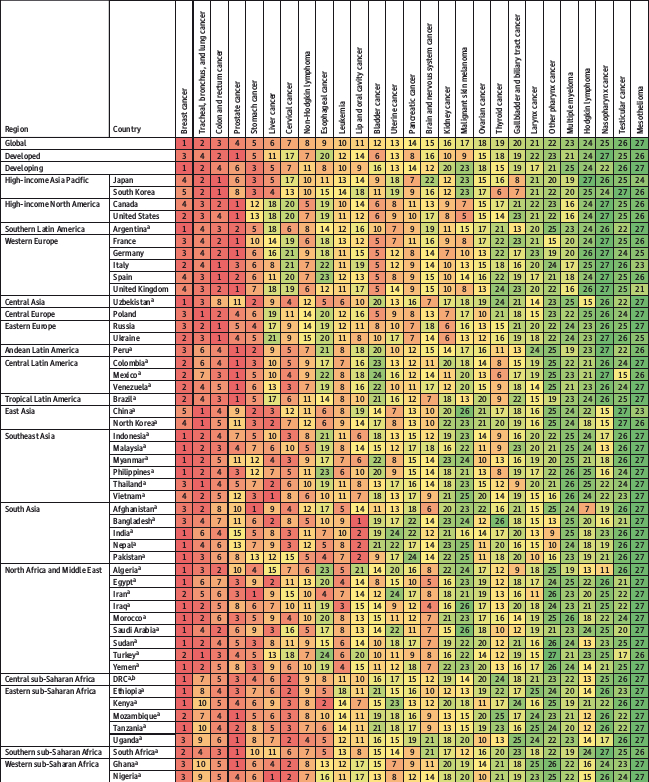
\includegraphics{cancer_incidents}
\end{figure}
\begin{figure}[ht]
    \caption{Cancers Ranked by Number of Deaths in Both Sexes, Globally, by
    Development Status, and in the 50 Most Populous Countries, 2013}
    \includegraphics{cancer_deaths}
\end{figure}

\subsection{Specific biomarkers}
An example of a single molecule biomarker is the prostate specific antigen
(PSA). This is a protein produced by the prostate gland in male humans. The
identification of cancer with PSA is simple, the higher the level of PSA,
measured in ng/mL (nanograms per milliliter), the higher is the chance of the
patient having prostate cancer \cite{cancerfacts}.

Today PSA is used for both identifying and evaluating the current stage of
prostate cancer. This biomarker can be found by analyzing blood examples from
patients, thus fulfilling some of the demands for a good biomarker, but not all
of them. It is easy to measure and easy to acquire, but not reliable enough to
be used as the only marker to identify and determine the stage or remission of
prostate cancer. The low grade of reliability comes from the fact that even
though higher levels of PSA shows higher chance of having prostate cancer,
prostate cancer is not the only reason to have elevated levels of PSA
\cite{cancerfacts}. Namely inflammation and enlargement of the prostate. Though,
a man with both of these cases may or may not develop prostate cancer.

So the conclusion for the PSA biomarker is that it is not reliable enough and
are causing faulty treatment of prostate cancer that may not even exist. Because
even if a patient has prostate cancer, it may not be harmful, promoting the case
of not taking any action against it at all. So there is need for a new
biomarker, or at least a better way to diagnose and predict the right treatment.

\chapter{Big data in bioinformatics and networks as a tool in cancer research}
\section{Existing biomarkers}
The PSA biomarker is over 20 years old \cite{psa-age}. Through those years, it
has been discovered other and better biomarkers for prostate cancer than PSA.
Among those, PCA3, which is detectable through urine samples from patients. It
also has the benefit of not being affected by the size of the prostate gland
\cite{pca3-size}. But still the results could be better. Therefore, it has been
tried to combine these two biomarkers in order to see if it is beneficial to see
the results from each biomarker in light of each other \cite{beyondpsa}. The
results from these tests is that they complement each other to a level of
significance that makes it compelling to analyze them both to diagnose prostate
cancer. It is important to point out that even if these biomarkers are not the
best at indicating if a patient has cancer or not, these biomarkers are good at
indicating progression and recurrence of prostate cancer.

In the cases of pancreatic, lung, breast, brain and overian cancer, the somatic
distribution of single-nucleotide polymorphisms (SNP) has a few altered genes
that occur with a frequency higher than 10\%, and many other genes that are
mutated occur with a frequency of 5\% or lower\cite{pathway-network}. On the
other hand, prostate cancer has relatively few SNPs and copy-number alterations
(CNA), so that kind of cancer is more likely to be driven by another somatic
variation, namely DNA methylation. Cancer driver genes can be detected by
positive-selection signals in the mutation pattern of genes in tumors, but there
is a drawback with this method. Genes that are less frequently mutated within
tumor samples might not be identified by a statistical analysis, even if they
might be functionally important. An alternative method is to use prior knowledge
of cellular mechanisms, and add this prior knowledge as attributes to genes
represented as nodes in a network. Then we can use graph algorithms to gain
novel information about cancer driver genes. Genes that is not listed as cancer
driver genes can then be assigned a status "guilt-by-association" if they have a
network-relationship with proven cancer driver genes.

But all of this is based on single genes or proteins. What if we looked at whole
networks as biomarkers? In this case, we will look at clusters of networks.

\section{High-throughput sequencing}
Today, rapid analysis of genes and proteins are made available through
Next-Generation Sequencing (NGS)\cite{ngs1}. Networks offers us an informatic,
algorithmic, visual and mathematical tool to study this bigger picture. This
project will integrate the opportunity networks offer to discover new biomarkers
in cancer. Through acquiring more data, faster than before, there now exists
databases with large amounts of information that is easy to access. This makes
room for building huge networks of proteins and genes, allowing for more
extensively and thorough assays to be done. For example, what if something that
is classified as a prostate cancer biomarker only is viable when proteins that
has not been classified as a biomarker, also is present?  Together they could
represent a more appropriate \emph{network cluster biomarker}. The amount of
data that can be analyzed also opens up for another more personalized approach
to each cancer patient. Finding patient-specific biomarkers could make a huge
impact on the quality of treatment \cite{personalized}.  

\section{Networks as a tool in cancer research}
Viewing the cell as a network of proteins and genes presents us with several
assumptions to make. A way of defining edges between nodes has to be
established. It exists several ways of doing this, but it depends on the
context.

Bayesian probability networks are one way of defining edges
\cite{bayesiannetworks}. It is based on the probability that if a node A exists,
then node B exists. That way it is possible to create networks based on the
assumption that if node A exists, then node B is 80\% likely to exist. Maybe
node C and D have a 100\% chance of existing if node B exists.  These
percentages represents how strong the edges between the nodes are, and makes it
able to construct a directed acyclic graph (DAG). It is important to note that a
true bayesian network can not be achieved through random observations. Rather
should some constant value(s) be introduced to be able to really measure the
effect of the other variables.

The way of defining edges in a network also determines what kind of information
that is possible to get from it. The different bio-databases has different ways
of calculating edges. Should the database alone define the edges? If the
database supply weights in the edges and/or nodes, should it be used, changed or
ignored? The final decision of how and in what way the edges should be defined
in this thesis has yet to come. 

\subsection{Pathways and networks} % malplaced??? TODO: SOURCE
Pathways are small networks of well studied processes where many areas are well
documented. Networks on the other hand are bigger and less explored, but when
properly analyzed, it might provide new information unknown to pathway systems.

Analyzing pathways and networks have an advantage over individual genes. They
may reveal information that comes from molecular events that covers multiple
genes or pathways. Aggregating this data can increase the chance of detecting
driver genes through statistical analysis. Also, information gathered through
pathways and networks may be enriched through genomic, transcriptomic and
proteomic data and create a more unified view of the tumor biology.

\chapter{Network clustering: Toward network based biomarker discovery}
Networks is the pre-processing of single gene prioritization that is necessary
in order to come to the next step, clustering of the network. Clustering is
about making a hierarchical view of a network to be able to look at the bigger
picture. The reason to group a network into clusters and rank them
is that the edges we create represents different connections. They can represent
function, probability of existence, interactions or contents of the cell
\cite{siri}. There is several algorithms to create clusters, and all need to be
researched in order to find the best suited one. The major differences on how
these algorithms work is centered around how they handle nodes and edges. For
example how the cluster is expanded, what density level it is aiming for, how
robust the algorithm is towards incomplete networks. It is feasible if the
cluster-making algorithm is easily, or even already implemented as an app in
Cytoscape. ClusterMaker2 is such an app and will be considered \cite{cm2}. But
there is faster cluster-creating algorithms than those implemented in
ClusterMaker2, an example is the SPICi \cite{spici} algorithm. So a possible
solution for Ranklust could be to implement the SPICi algorithm into the
ClusterMaker2 app, in order to reuse most of the code that represents the GUI,
single gene prioritization and network creation. In addition to the
cluster-creating algorithms, there is a need for cluster-ranking algorithms.
They should be ranked in the order of being a cluster biomarker, more specificly
described, a cluster biomarker for prostate cancer. The idea of clustering is to
identify relationships between cancer driver genes and genes not related to
cancer that reside within the same cluster. Since a cancer driver gene and a
gene that has not been proved to be a cancer driver gene has a relation, the
latter might play a role in cancer. These genes will be identified as candidate
biomarkeres for prostate cancer. This was mentioned earlier as the
"guilt-by-association"-principle.

\chapter{Ranklust: An implementation to rank clusters}
\section{Cytoscape}
Cytoscape is the open-source software platform the Ranklust app will be
developed on. Its main purpose is to visualize molecular interaction networks
and biological pathways.  It is easy to integrate \textbf{\textit{Apps}} and
even combine multiple apps to solve new problems, given that the source code of
the apps is available or that it exists an easy way of piping results from one
app to another. 

The goal of Ranklust is to rank the clusters in the network. Apps taking care of
making the networks and creating clusters already exists, so Ranklust will only
concentrate on the part that ranks the clusters and visualizes the results to
the user of Cytoscape.

\section{Programming language}
The reason to choose Java above Python, Perl or other popular programming
languages in bioinformatics is simply because of development experience. Java
8 is known for being this big bloated enterprise programming language, and
Python as the fast and easy mockup tool to develop good programs fast. Python
also has big biological computation libraries like \emph{Biopython}
\cite{biopython} and sklearn\cite{sklearn}, that makes it easy to build your own
standalone apps.  Though when used in a bigger environment as Cytoscape, Java
shines, having sturdy packaging and modelling standards. The Cytoscape community
is big, alive and has standards for how the architecture of apps should look
like. The community promotes this through the use of the \emph{OSGi} standard
\cite{cytoscape-osgi}.

Formatting and cleaning the data that Ranklust will provide and export out of
Cytoscape is done in Python 2.7\cite{python}. As mentioned over, it has many
small libraries that can help with the bioinformatics part, and the scripts
needed to format the data will rarely exceed over 100 lines of code.
Third-party libraries like pandas\cite{pandas} and numpy\cite{numpy} will
support the formatting and cleaning of data.

\section{OSGi and design patterns}
Developing OSGi software promotes modularization \cite{modularization} of the
code and increase the probability of the app being launched as an official
Cytoscape app; in addition to provide other developers with the possibility of
reusing my modules in their own apps. Also, it seems like Java 9 is aimed at
making it easier to modularize apps along the lines of the OSGi
standard\cite{jigsaw}, so it might be easier to refactor an application in the
future from Java 8 to Java 9 when the architecture already is in place. There
exists several design patterns that could prove to be useful in the development
of Ranklust. Another strategy to follow may not be a direct design pattern
\cite{designpattern}, but more of a collection of them, and it is the clean
code principles by Robert C. Martin \cite{cleancode}. Going against the coding
principles promoted by the Cytoscape app community and exclude the use of OSGi
modules will not be done, but third party Java libraries that is not OSGi-ready
will be used, namely the JUNG library\cite{jung}.

\chapter{Databases}
\section{Databases for network information}
Which databases to use has to be considered. The reason to use databases is
because they have information about how protein and genes form a network based
on how they interact with each other. The initial database candidates in
Ranklust are iRefIndex \cite{iri}, GeneMania \cite{gm} and STRING \cite{str}.
These databases all have in common that it exists Cytoscape apps made to use
these databases. STRING however, does not have any repository available through
the Cytoscape app store, so interacting with the database through a new app in
Cytoscape without making new plugins may be difficult. On the other hand, both
iRefIndex and GeneMania have their repositories easily available to the public
together with decent documentation. However, the difference between them is what
they contain information about. iRefIndex contains data about protein-protein
interaction (PPI), while GeneMania contains data about genes.

Since proteins come from genes, GeneMania can also give us some information
about proteins. The open-source plugins in Cytoscape to communicate with the
databases are iRefScape \cite{iridb} for iRefIndex and GeneMANIA \cite{gmdb}
for GeneMania.

\section{Neo4J}
A problem we had with the Neo4J\cite{neo4j} database is the dump it creates.
The dump creates a single Cypher\cite{cypher} commit for the whole database.
This way, if anything goes wrong while importing the data, it will get rolled
back. It hinders faulty data and relationship between several parts of the data
to be imported into the database. The problem with a single commit to import
the data is the required memory. The personal computer used in this thesis and
the computers at University of Oslo that we have access to did not have enough
memory to import the database as a single commit in Cypher. Splitting up the
dump to several commits does not work without quirks. It conquers the memory
problem, but the way the relationships are created from the Neo4J dump requires
the import process to be done in a single commit. A way to fix this is either
not to use Cypher queries as a way of importing the data, but instead use
GraphML\cite{graphml}. Another way is to refactor the Cypher dump so that the
creation of relationships does not need to be done in a single commit. We will
use both ways, because not being able to use the Cypher queries because of too
little memory will most likely be a problem for several people and not just me.
Using GraphML is good for exporting data from Cytoscape and from the database,
but interaction between the two of them while performing the algorithms is not
feasible at the time.  The last drawback is where Cypher queries are good,
because it exists plugins that aid in using data from the database directly in
Cytoscape. So initializing a database for testing could easily be done with
GraphML, and then use Cypher queries to instruct a database to perform
computations on the data.

Creating a script to refactor the Cypher queries does not only help in regards
of using the data with Cytoscape, but also for everyone using a Neo4J Cypher
dump to create a database and does not have much memory. A problem that might
come up is performance. Because the current way of creating relationships use
node labels in Neo4J and it takes only a single line to create a relationship
between two nodes. If we refactor the relationship-part of the Neo4J dump, it
will increase to a two instruction query. Firstly, two nodes has to be found
based on their indexed node name, which will relate to the protein/gene name.
Secondly, we do the same thing that was done before the refactor, we create the
relationship between the two nodes. The difference between the old and the new
way of creating the relationship is how the nodes are found. The Neo4J dump
creates temporary node variables prepended with an underscore and an integer ID.
These ID's only exist within the commit the nodes are created. So splitting
creation and relationship-making leaves us with worthless IDs that does not
refer to any known node. That is when Neo4J tries to be smart and then creates
new nodes based on the underscore ID and then creates a relationship between
them. The end result, two new nodes that only contains the undescore IDs. So the
refactored version aims at matching the underscore IDs in the relationship
creation to the node creation, and to replace them with the name of the nodes
instead of the temporary underscore ID. But as mentioned, matching the nodes
with the name takes up more time and performance might be an issue. For
comparison, with a Cypher dump of 4,500 lines, it takes about 20 seconds before
the query engine gets a stack overflow error from too little memory (4GB
memory). With GraphML, an XML file with 250,000 lines takes under 1 second to
import and it gets relationships right without any form of refactoring.

\section{Other database technologies}
Other databse technologies like SQL and NoSQL has not been researched in this
thesis to be used with Cytoscape or graph algorithms regarding 

\part{Images testing...}
\label{pa:images}



\part{The project}
\label{pa:project}
\chapter{Workflow}
\section{For researchers}
The way researchers will work with Ranklust is pretty simple. Step 1 and 2 will
only be required the first time the researcher want to use this app to solve
his/her problem. The rest has to be done every time, unless a previous session
of CytoScape is loaded with more developed results.

\begin{enumerate}
    \item Install CytoScape
    \item Install clusterMaker2 plugin through CytoScape App manager
    \item Upload the network to be clustered and ranked into CytoScape
    \item Use clusterMaker2 to cluster the network
    \item Use the Ranklust-part of clusterMaker2 to rank the clusters
        \begin{enumerate}
            \item Decide what to score the clusters on
        \end{enumerate}
    \item Use the Ranklust-part of clusterMaker2 to visualize the rankings
\end{enumerate}

Step 6 should show the researchers the ranking of clusters based on what
attributes they wanted to include in step 5a. This ranking represents cluster
biomarkers. The score of the clusters and the order they are ranked in will
decide the state of the patient. State of the patient can be many different
things and what the rankings will mean to the researcher is not yet final. It
will be a new indicator, a biomarker, and information about what it means has to
be gathered empirically through clinical research.

\part{Cytoscape} % Make this a subsection in "The project" part
\label{pa:cytoscape}
The structure of the code in Cytoscape follows the already established structure
in the ClusterMaker2 plugin. This is to make it easy to maintain for the other
contributors of ClusterMaker2. At the same time, the code is modularized enough
to make it easy to extract the code, in order to make a separate plugin. The
motivation for having a separate plugin to rank clusters in Cytoscape gets
bigger if ranking clusters provides useful information, in regards of
discovering cancer.

Adding new ranking algorithms should be easy both to implement and unit test.
Where the algorithms should be placed and how to connect it to the rest of the
GUI in order to choose it, should be a no-brainer. Unit testing of the
algorithms should be possible without using the GUI. So all of the logic in the
algorithms should be excluded from the GUI. If it is not excluded from the GUI,
testing the algorithms would require menu interaction and automatization of
testing goes out the window. Every test should be able to just run in the
terminal without launching Cytoscape.

The "Factory" design pattern % reference
is used in a original way in ClusterMaker2, and for the ranking cluster
algorithms it is done a little bit different.  The GUI will not be responsible
for knowing every available algorithm, it will be the algorithm factory's. The
GUI's way of knowing which algorithms the user should be able to choose from,
will be to ask the factory for a list of all of the available algorithms. This
is an example that shows by separating the amount of components that have
knowledge about a specific piece of information, it becomes easier adding new
features. If the GUI also would have to construct a list by itself about the
available algorithms, in addition to the factory, we would end up making changes
in two places instead of just one. Twice the work for just one change - adding a
new algorithm.

%%%%%%%%%%%%%%%%%%%%%%%%%%%%%%
%%%% IMPLEMENTATION START %%%%
%%%%%%%%%%%%%%%%%%%%%%%%%%%%%%
\chapter{Implementation}

\section{Intro}
The \textit{clusterMaker2} documentation for implementing new parts that is not
directly connected with clustering algorithms is non-existing (cite
documentation!). So I will make a "walk through" of how to do it and how I did it.

\section{Preparations}
The POM-file has to be updated because libraries connected to the pdf exporting
functionality is outdated. Updating the libraries, imports and the usage of
these libraries in the source code is enough to make the whole project compile
at the mentioned date.

\section{Registering a service}
In order to make it easy to implement new cluster ranking algorithms, a new task
factory for the ranking of clusters is required. It has to be registered as a
service to make it visible to the GUI menu, aswell as maintain the \textit{OSGi}
standard of components added to the \textit{clusterMaker2} project. Also,
creating a standalone plugin at a later stage will be easier if Ranklust is
properly compartmentalized.

Registering a new service listener is a way of keeping the Ranklust part out of
clusterMaker2. Though, it is still packaged within clusterMaker2's API, so that
it does not become a mess, if extra functionality is to be implemented while the
plugin resides within clusterMaker2.

\section{GetNetworkClusterTask}
ClusterMaker2 already has some REST (insert: reference to REST services +
explanation). It is used in Ranklust as a way of getting the clustering results
without changin the previous code. Though, there is a flaw in the REST service.
If the clustering algorithm you want the results from is not the last clustering
algorithm that was run on the network, it will not be able to get the results.
For now, this will stay as it is, but it should be brought up for discussion to
rather look up the table of the nodes instead of the table of the network, in
order to get the clustering results. This is because the table of the network
can only hold a single value for clustering algorithms, which will either be
nothing, or the last algorithm run on the network. The drawbacks of looking up
the table of nodes instead is the time it consumes. But the time consumed to get
all of the nodes with a specific clustering result attribute will take a shorter
time than to rerun the algorithm you want to have the results from. A third
solution can be to just ignore the algorithm used to cluster the network, as it
should not have anything to say for the ranking of the clusters. This may end up
being the final solution, as it easily can be viewed as a more "sane" (formulate
this in a different way). This option requires a new REST function to be added
to clusterMaker2. As a whole, it is highly possible that this new REST
functionality should replace the existing one. The argument to replace the
already existing algorithm is that REST functionality should hide state and
implementation from the services using the REST service to get data. The way it
is now, this is not true and it should be changed anyway.

\section{Tables vs pure OO}
One thing in particular that deserves to be mentioned is the way networks are
handled. The \textit{CyNode} objects themselves does not contain much. This is
because all of the information is saved in the form of plain cells in a
spreadsheet. This may at first seem like a way to make it easy to show
information to the user, but it is also a way of working more efficient with
network data (insert: reference to working with tables on networks is
efficient). Creating objects with attributes for each node in a huge network
will increase the amount of overhead by a pretty noticeable amount. Working with
all of the information in the way of a spreadsheet with rows and columns
includes a decrease in overhead. A new node is a new row, so in relation to
build the network structure, it is not a difference to speak of.  The difference
comes in when the nodes have several attributes. 

In a table or spreadsheet, attributes can be represented as a single column and
be created once for the whole network, instead of once for each node object
created. This assumes that getting the objects out of the table is possible by
either indexing on a number for arrays, or a unique string for map structures.
The result is both a lookup, insertion and deletion time of O(1) (insert:
reference to Big-O notation).  These times is as law as the Big-O notation goes
in terms of speed related to the size of a collection inside a data structure.
So both the creation of objects goes down, and the retrieval of attribute
information is as low as it is possible to get, when we choose to represent the
time by Big-O notation. The only drawback with this implementation is that there
is no current type of wrapper around the row and column system. So the retrieval
of information is not done the most intuitive way. But this is the way Cytoscape
works as a whole, so changing the way this works is either done through changing
the Cytoscape source code, or implementing a wrapper as a standalone function
inside clusterMaker2 or as a standalone plugin.

\section{Single value ranklust}
A simple, but effective way of ranking clusters, is just to add together the
biomarkers values and sum them up in each respective cluster. This will tell us
which cluster will have the most cancerous genes and proteins. It is not very
advanced, but an analysis show how effective it is. An alternative is also to
add scaling to the values. Should clusters with a large amount of biomarkers
receive a bonus because of the sheer amount? Should values alone be scaled
exponential in order to magnify the differences between more and lesser
cancerous biomarkers? This will be tested in the final stages of single value
ranking in Ranklust. But as a beginning, the results will come from a pure
additive algorithm.  The more advanced ones will be implemented only if the
additive algorithm show promising results.

\section{Multivalue Ranklust}
Multivalue ranking of clusters creates a larger context. More data can help
making more fine tuned results and get the validation of ranking clusters to
find biomakers, hit the significance ceiling of 95\% certainity. 
% Fix this sentence!
The question here is how should several values be combined in order to create a
single value score to rank the clusters by? The best way should be to list every
attribute to the user, and present them with options as to how the values should
be scaled. An extra option could be how to scale the values in relation each
other. The first way is the simplest way to implement so it will be tested
first. And as with the single value ranking, if the first scaling of each
individual value shows promising results for multivalue ranking, the values in
relation to each other will be considered as a way of producing more accurate
results.

\section{How to get the clusters}
As of now, the SimpleRanking algorithm for ranking the clusters has to have
access to the cluster results inside the clusterMaker2 source code. The
alternative is to work directly on the Cytoscape tables containing the same
information. The drawback working on the Cytoscape tables is the need for going
through every single node in the table in order to add it to a cluster, which is
something the source code in clusterMaker2 can serve with a single
\textit{getter} method. The drawback using the clusterMaker2 code and not the
Cytoscape tables is that the getter method to clusterMaker2 demands knowledge in
the SimpleRanking algorithm of the cluster algorithm that was used. Coupling
these two object classes together is not necessary, because of the two mentioned
ways of completing this, and the getter method used is actually implemented with
the intention of creating a REST API \cite{rest-api} for applications outside
Cytoscape. A third way could be to implement a way for all of the clustering
algorithms to save their results as a \textit{List<NodeCluster>} list. Once
again this just moves the problem a bit around and we will end up with a good
amount of duplication code to the REST API method of getting the clusters. Then
again, having the REST API getter rely on the \textit{List<NodeCluster>} getter
could make for a cleaner solution. This is definetively more work and requires
every new clustering algorithm to implement a way of creating these node
clusters.

Creating the list of node clusters every time a ranking algorithm should run is
maybe not such a bad idea. Atleast when we consider that having every clustering
algorithm saving its results could result in massive memory constraints. Every
node in the node cluster list should only be a java object reference to a node
in the Cytoscape table. A Java object reference consists of 8 bytes
\cite{java-reference-size}. So we will end up having 8 bytes for every node in
the list to a single cluster. Also, to organize it properly, a list of the
clusters also has to wrap round all of the clusters, adding another 8 bytes per
cluster entry. One simplification can be made, which is using the indexes in the
list as a cluster score attribute from the cluster algorithms. That could
exclude clustering algorithms that produce more than a single score as a result
of the clustering. A sample clustering with the affinity propagation algorithm
produces 839 clusters. That is 6,7 megabytes for only the cluster entries in the
outer list. From the same results, the biggest cluster consists of over 700
nodes. That is 5,6 megabytes of memory on a single cluster. Total amount of
nodes in the network is ends up using extra memory of 89,7 megabytes. And that
is just per clustering algorithm.

\section{Edge attribute information}
In order to work with attributes in the edges, you would think that an
additional datastructure like a simple java class like \textbf{Map} or a class
which inherits attributes from the Java \textbf{Set}-class\cite{java-set} would
be preferrable. However, this is not necessary, as Cytoscape provides both the
source and target node in an edge, together with methods to get the primary key
from both of them. This allows us to index the node table and get the cluster
information in O(1) time.

Recipe for working the nodes and edges. Only the edges require step one, nodes
can start at step 2.

\begin{enumerate}
    \item Find common or best ranked cluster between two nodes (one edge).
    \item Add score to the cluster
    \item Repeat step 1-2 for every edge
    \item Sort clusters based on rank and create a column to represent the score
\end{enumerate}

Step 1 is the thing that will take extra time for the ranking algorithms
including the edges.

There is also a question on how we should add the edge scores to the cluster.
Should we add the score of the edge when we visit both the source and the target
of the edge? Only from when we visit the source, or only the target? Should the
user be prompted about this? Should the algorithm take into account if the edge
are directional. Or maybe the user should always provide edges in a specified
form. A form that says always specify the source node first, then the target
node. Maybe it should be specific to the attribute we are working with. The ways
to go here are so many. So many that I will just specify one way, and stick to
it. 

\subsection{Edge handling}
When iterating over the list of edges in the network, check first the source
node for a match, then, if it does not have a match in the node table, look
after the target node. Then add the score to the cluster. I assume that the
direction, if any, is from the source node to the target node. That way, the
score only gets added once to the cluster per edge and it does not have anything
to say if it is the source or target node. The user should have responsibility
for having the edges directed as from the source node, to the target node, if
a direction exists at all.

%%%%%%%%%%%%%%%%%%%%%%%%%%%%%%
%%%% IMPLEMENTATION END %%%%%%
%%%%%%%%%%%%%%%%%%%%%%%%%%%%%%


\part{Procedure}
\label{pa:procedure}
The secretome values of genes can be expressed by a single integer value,
though, for compatibility reasons Ranklust will require double values. The
clustered network can be constructed with an AP, short for Affinity Propagation,
clustering algorithm \cite{affinity-propagation}. Affinity propagation
clustering concentrates on the nodes in the network that are binding the rest of
them together. Using affinity propagation for clustering will produce results
that represent a grouping of nodes that are coupled by seemingly unimportant
nodes to most clustering algorithms. But the AP algorithm is good at expressing
nodes that are not highly connected to many nodes, but rather the nodes that are
binding other highly connected nodes together. This results in bigger clusters
that can be a target for methods that cure cancer by severing the interaction
between biomarker genes.

It is also discussed how AP performs versus Markov clustering (source, both
markov algorithm and the "vs" paper). And since Markov algorithm performs better
on protein interaction, it will also be used to cluster the networks. An
analysis between the rankings that come from the Markov and AP clusterings will
be performed, which hopefully will give concrete results as to the pro's and
con's of each algorithm. Some questions should be raised as the analysis is
done. For example, is both of the algorithms good, but have different uses, even
if they are not directly involved with the ranking done after the clustering?
Are either AP or Markov useless for a particular type of ranking afterwards?

The information provided through the whole process from what type of nodes
(protein or gene), interaction between the nodes and what kind of biomarker we
want to identify are all factors that will have a great impact on how all of
this should be combined. The order of operations on the network will also effect
the result. For example, AP clustering may create a few big clusters and many
small ones. At this stage, the results will consist of the biggest clusters
constructed from AP clustering that has focus on pure connection between nodes
and not their attributes. At this point, the cluster ranking algorithm of
Ranklust will be run in order to produce a picture of potential biomarkers. This
picture is the first and simplest step that will be used as a result for an
analysis. The analysis in this thesis will focus on validating the cluster
ranking scores as ways of indicating potential biomarkers. 

In order to validate the scores, I will need to know the state of the patient
that the data to create the network came from. As there is no use to just
generate results without knowing what they show. They might show connections
between them, but without some sort of context the results are useless. The
context needed is not very high, but the results from the ranking should be
tested for several purposes. For example, is biomarkers from ranking of clusters
best for disease disposition, screening, diagnostic, prognostic, prediction or
monitoring cancer. I will aim for screening, diagnostic and most of all
prognostic usages. As mentioned earlier, the prognostics of prostate cancer
often results in 50\% of patients receiving treatment that was not needed.


\part{Results}
\label{pa:results}
\chapter{Ranklust as a tool for researchers}
\section{The planned workflow in general}
First off is the general workflow: (\ref{fig:ranklust-workflow})
\begin{figure}
    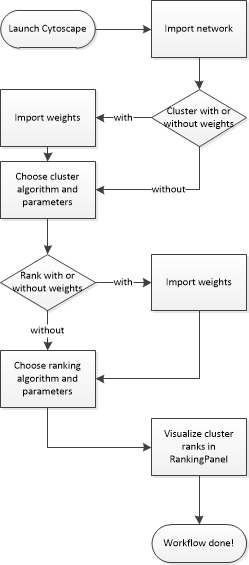
\includegraphics[scale=0.8]{ranklust_workflow}
    \caption{General workflow of using Ranklust to rank clusters}
    \label{fig:ranklust-workflow}
\end{figure}

\section{Detailed walk-through of using Ranklust}
To go into more detail, here is the startup screen (\ref{fig:startup}) that the
user is met with after launching Cytoscape. This assumes that clusterMaker2 with
the Ranklust contribution is already installed in Cytoscape.
\begin{figure}[H]
    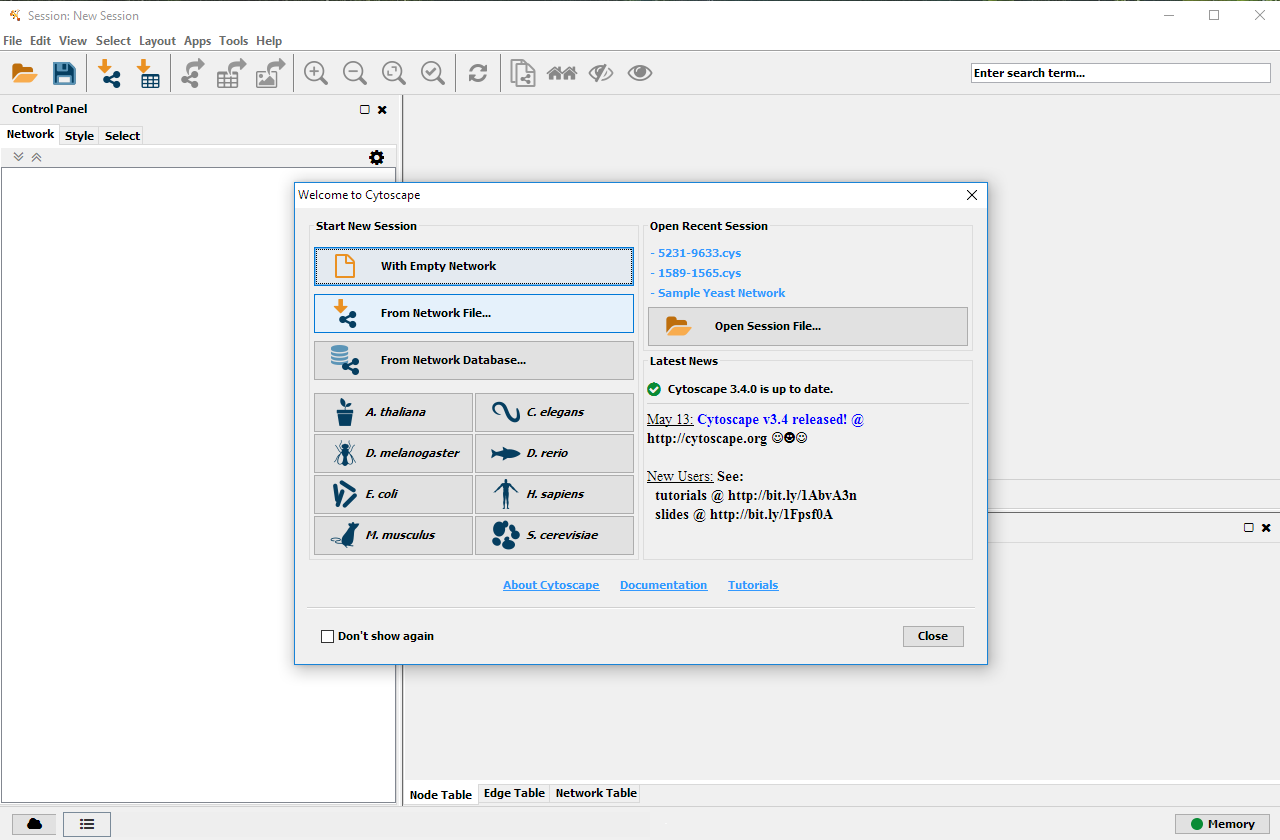
\includegraphics[width=15cm]{1-startup}
    \caption{Startup screen greeting the user at Cytoscape startup}
    \label{fig:startup}
\end{figure}

This screen (\ref{fig:import}) is what opens up after opting to import a network
and choose a network file consisting of a header that represents source and
target node columns, a\_alias and b\_alias. The names for the columns does not
have to be exactly a\_alias and b\_alias, but there should be some header
information indicating a source and target gene/node. Having no header in the
data imported into cytoscape is not a problem, but it requires the user to
explicitly specify this in the "Advanced Options" menu and check off the "Use
first line as column names" option.
\begin{figure}[H]
    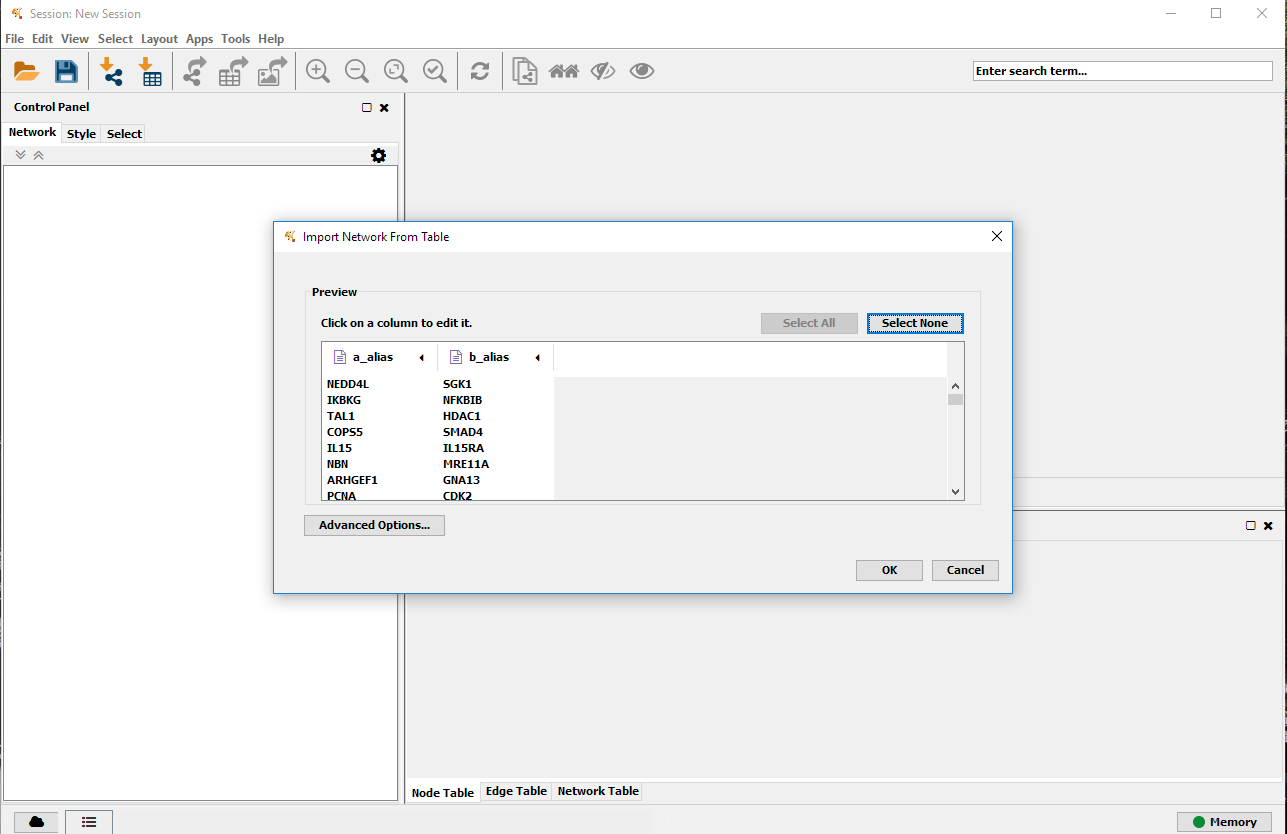
\includegraphics[width=15cm]{2-import}
    \caption{Importing a network into Cytoscape}
    \label{fig:import}
\end{figure}

It is important to tell Cytoscape which column is considered as the source and
target column, as shown here. In this thesis, approved gene symbols from HGNC
has been the primary key identifier in both source and target column.
\begin{figure}[H]
    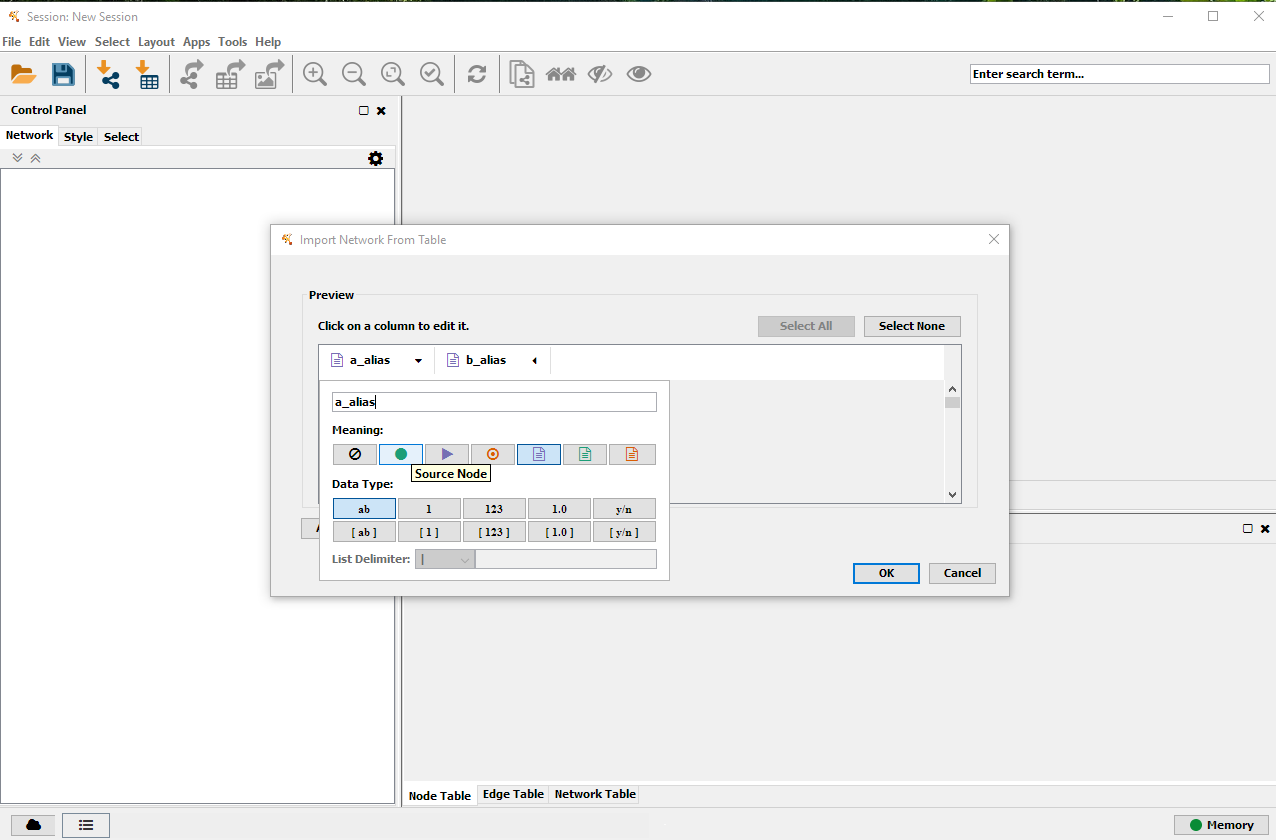
\includegraphics[width=15cm]{3-nodes}
    \caption{Choosing source and target nodes of the interections in the network}
    \label{fig:nodes}
\end{figure}

This is how Cytoscape looks after importing the network and it has finished its
standard style layout algorithm, which happens automatically after clicking "OK"
in the previous screen - having set everything to the correct settings.
\begin{figure}[H]
    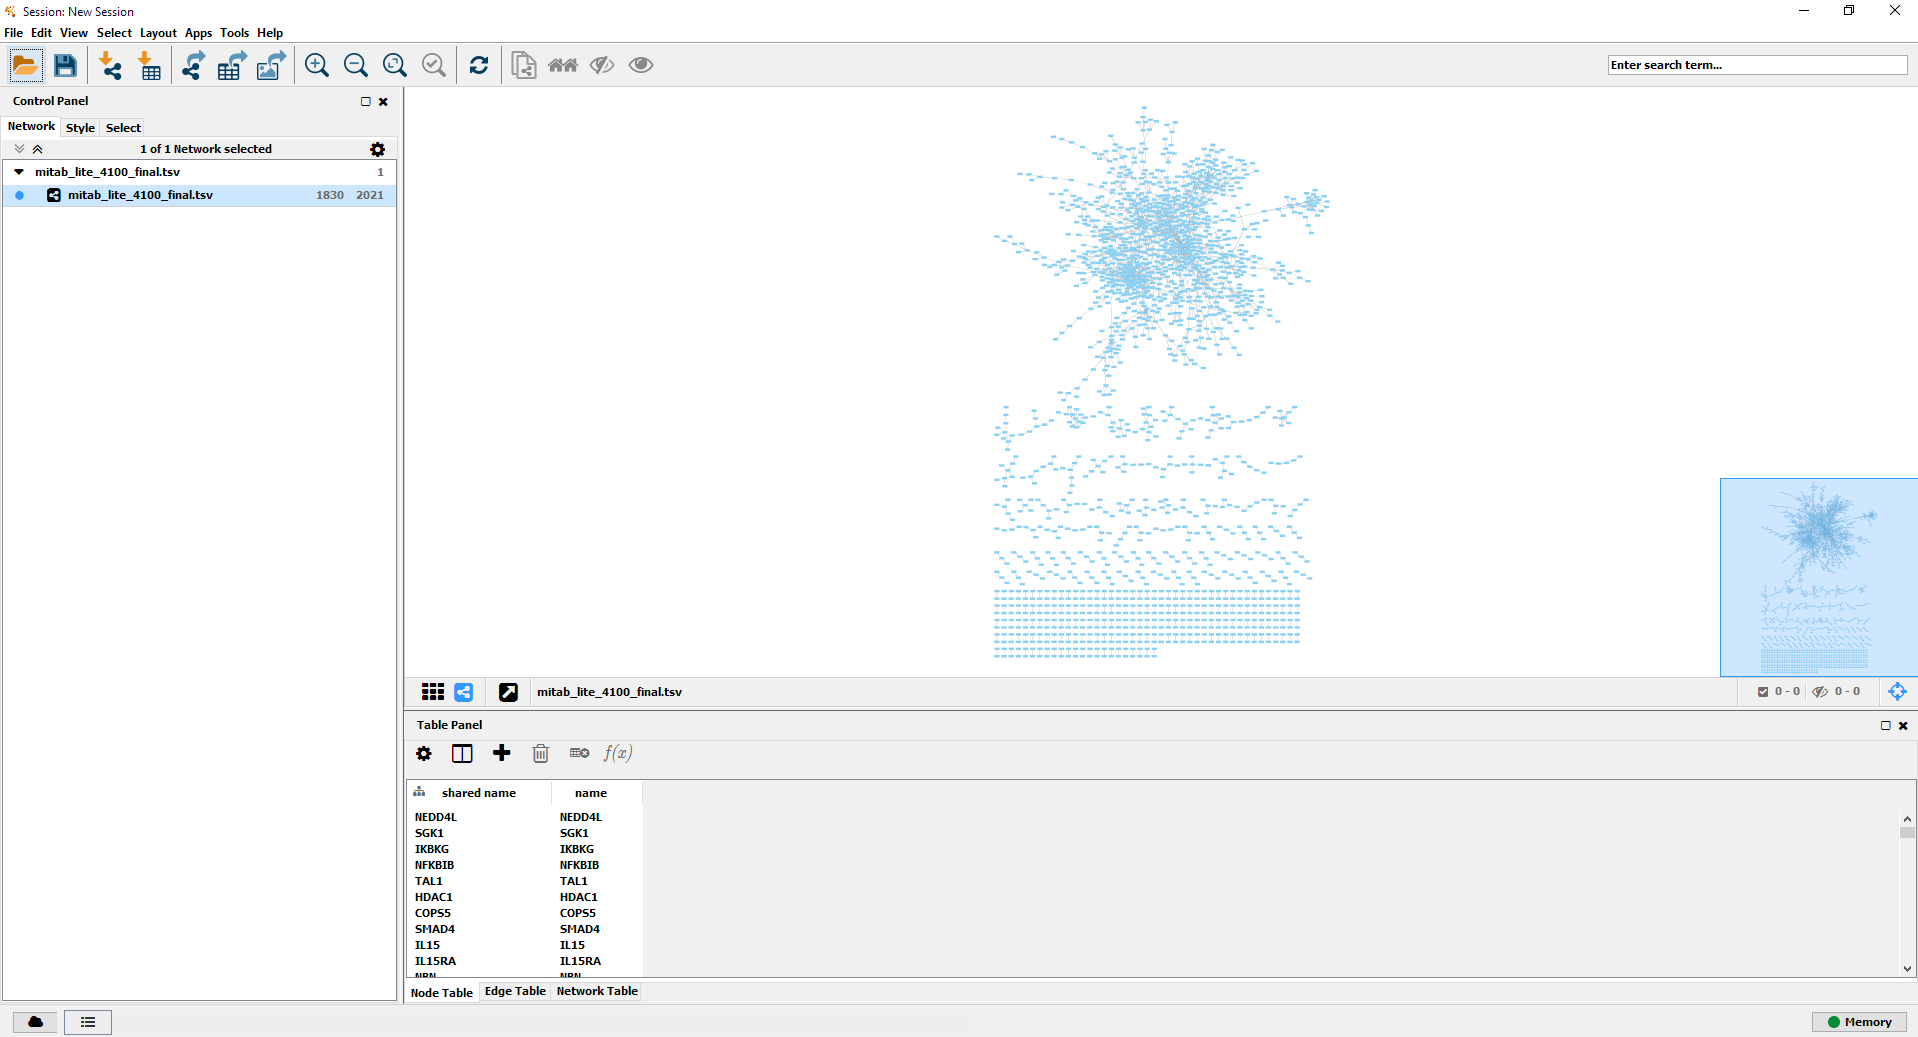
\includegraphics[width=15cm]{4-imported-network}
    \caption{Cytoscape view after network import has finished}
    \label{fig:imported-network}
\end{figure}

If the user wishes to weight nodes for clustering or the ranking of them, it is
possible to do this with the "Import Columns From Table" function. Adding prior
scores to the iRefWeb network that was created, the file representing the table
to import scores from had two columns, "geneName", which representet the gene
symbol and was the primary key for matching the score with the right row in the
Cytoscape tables, and "score", which contained scores between 0 and 1.
\begin{figure}[H]
    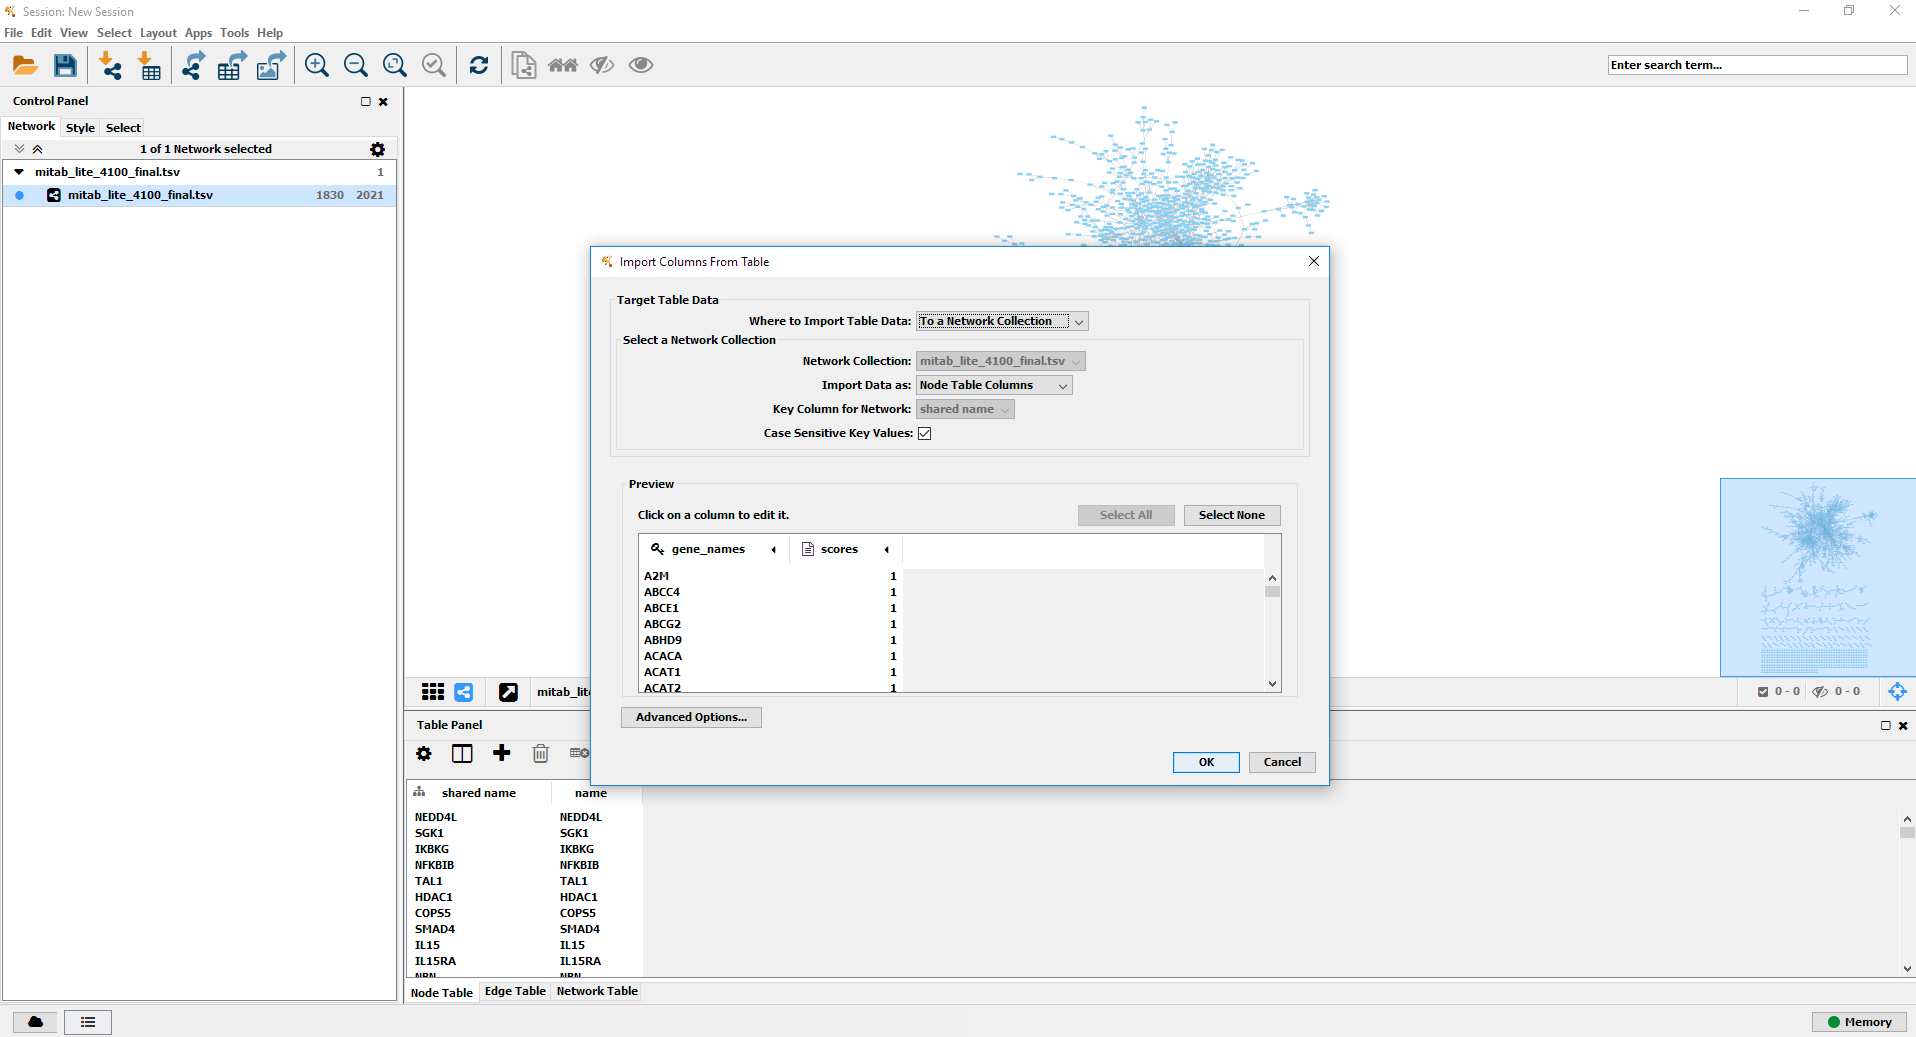
\includegraphics[width=15cm]{5-import-table}
    \caption{Adding prior scores to the network}
    \label{fig:import-table}
\end{figure}

To cluster the network, the user has to access the \textit{Apps} menu at the top
in the toolbar of Cytoscape. In clusterMaker2 there are three rows belonging
to the plugin. \textit{clusterMaker} row, where the clustering algorithms are
located. \textit{clusterMaker Ranking} row, where Ranklust's cluster ranking
algorithms \gls{maa},\gls{mam},\gls{pr},\gls{prwp} and \gls{hits} are. Finally,
the \textit{clusterMaker Visualizatons} row, where different visualizations in
clusterMaker2 can be queried. This row is also where option to visualize
Ranklust's ranked clusters resides.
\begin{figure}[H]
    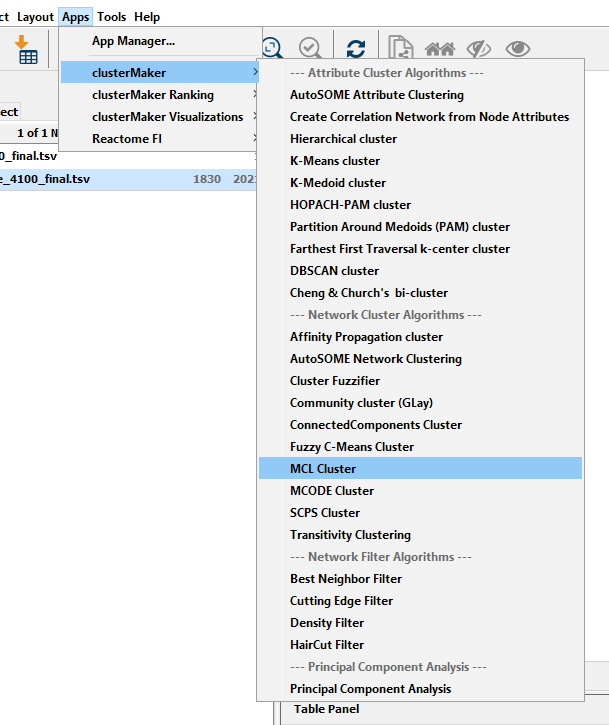
\includegraphics[width=15cm]{6-cluster}
    \caption{Choosing the MCL cluster algorithm in clusterMaker2}
    \label{fig:cluster}
\end{figure}

This is the view after clusterMaker2 has run the \textit{MCL cluster} method on
the current network. As seen on the left side menu, a new network has been
listed. This network only appears if the user sets the "Create new clustered
network"-option in the clustering parameter dialog that appears after choosing a
clustering algorithm from the clusterMaker2 menu.
\begin{figure}[H]
    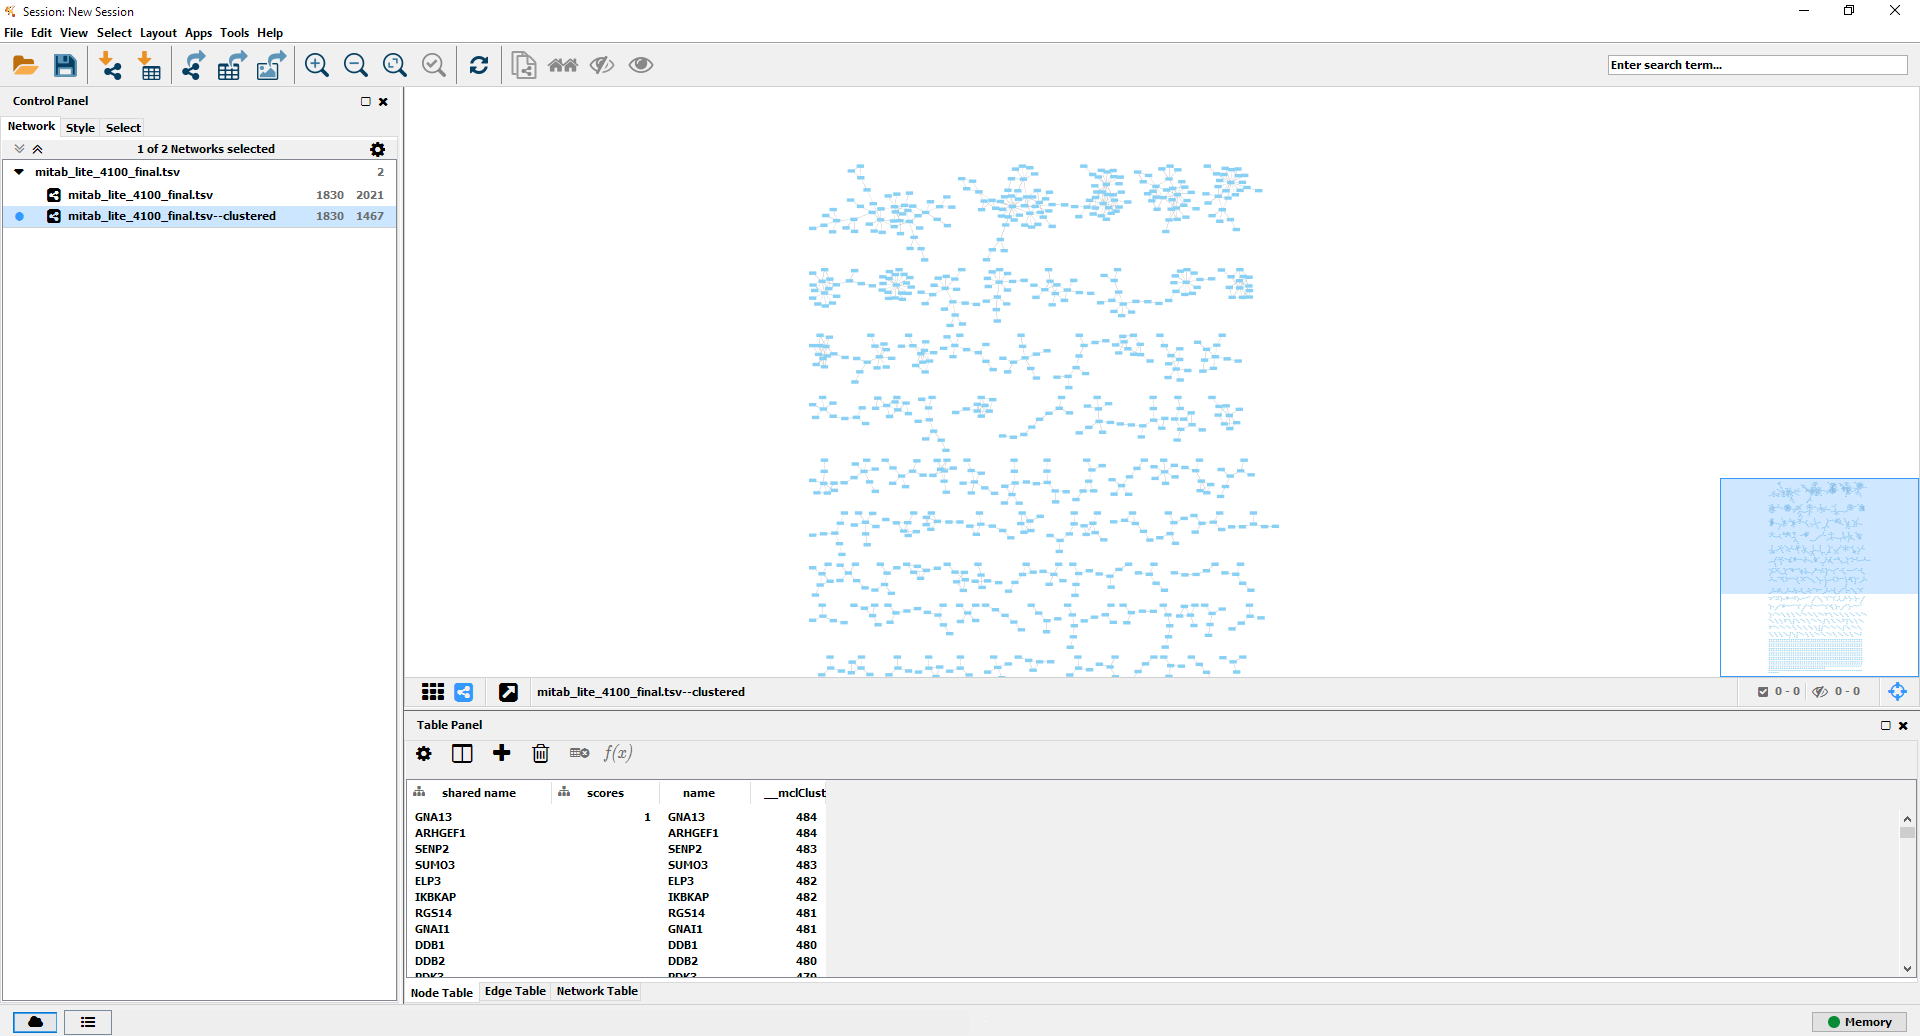
\includegraphics[width=15cm]{7-done-cluster}
    \caption{Network view of the clustered network created by MCL - note the
    added column in the Node Table}
    \label{fig:done-cluster}
\end{figure}

Here the cluster ranking algorithm menu is shown.
\begin{figure}[H]
    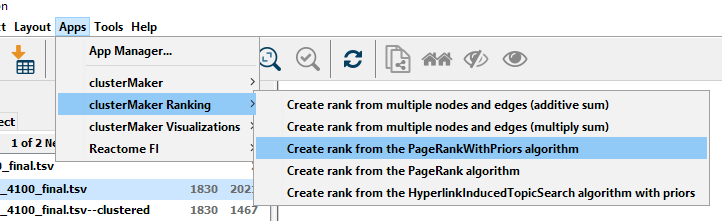
\includegraphics[width=15cm]{8-choose-ranking}
    \caption{Choosing the PageRankWithPriors (PRWP) ranking algorithm to rank
    the clusters in the network}
    \label{fig:choose-ranking}
\end{figure}

The "Create rank from the PageRankWithPriors algorithm" (\gls{prwp}) was chosen
as the ranking algorithm. Node and edge attributes can be combined by the user
in through simple selection. Selecting no attributes will cause \gls{prwp} to
not calculate scores at all. If the user does not want to use attributes to rank
the clusters, but still use PageRank, the "Create rank from the PageRank
algorithm" (\gls{pr}) algorithm should be used.
\begin{figure}[H]
    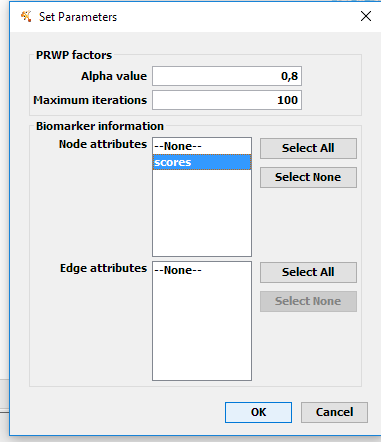
\includegraphics[width=15cm]{9-pagerank}
    \caption{Setting the PRWP parameters before executing the algorithm}
    \label{fig:pagerank}
\end{figure}

If the user is interested in visualizing the ranks, it is possible to click the
"Show results from ranking clusters" option in the visualization menu of
clustermaker2. No menu will appear after that, but rather will Cytoscape open
a loading dialog similar to when clustering and ranking algorithms has been
tasked to start. After the loading dialog is finished, the results panel for the
ranked clusters will be shown.
\begin{figure}[H]
    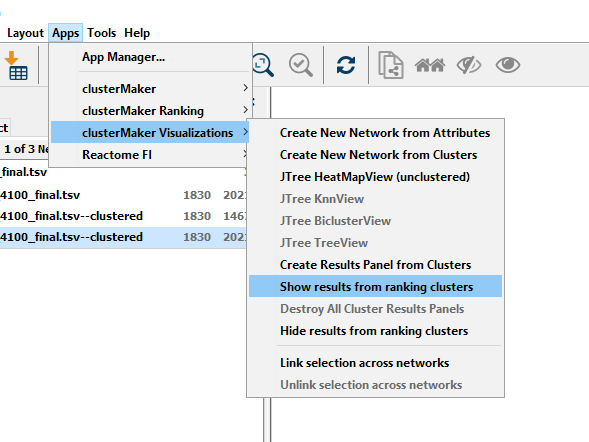
\includegraphics[width=15cm]{10-show-results}
    \caption{Choosing to visualize the results after the PRWP algorithm has
    finished}
    \label{fig:show-results}
\end{figure}

Here is the results panel displaying the ranked clusters from top to bottom,
descending scores. The title for each results panel is formatted as in the
example.
\begin{Verbatim}[fontsize=\scriptsize]
[<clustering algorithm>]{<ranking algorithm>}(<network name>)
\end{Verbatim}
So with MCL clustering, \gls{prwp} ranking and the
"mitab\_lite\_4100\_final.tsv--clustered" network, this is what the title
becomes:
\begin{Verbatim}[fontsize=\scriptsize]
[mcl]{PRWP}(mitab_lite_4100_final.tsv--clustered)
\end{Verbatim}
As seen in the title. The coloring has been discussed earlier.
\begin{figure}[H]
    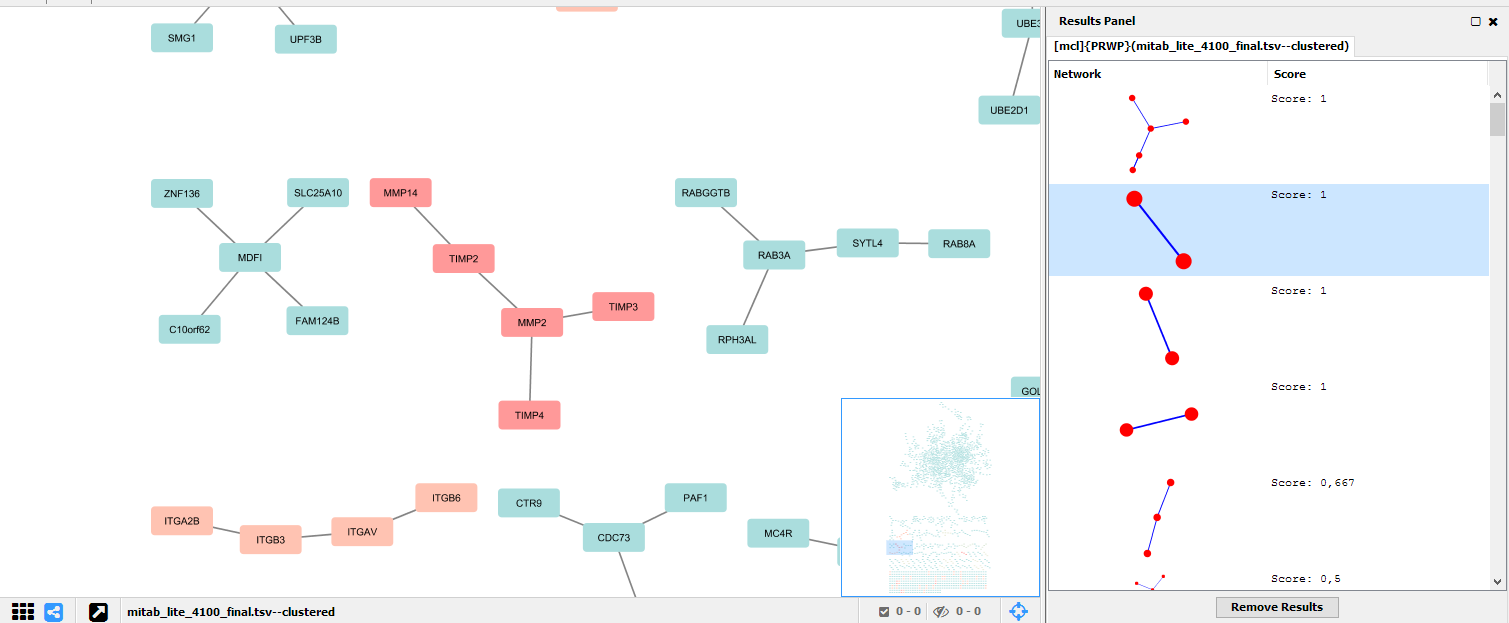
\includegraphics[width=15cm]{11-result-colors}
    \caption{The visualization of the ranked clusters are finished, both colored
        nodes in the network and the results panel on the right side is
    displayed to the user}
    \label{fig:result-colors}
\end{figure}

Here is an example of how the clusters change color when the same cluster is
selected from the results panel menu.
\begin{figure}[H]
    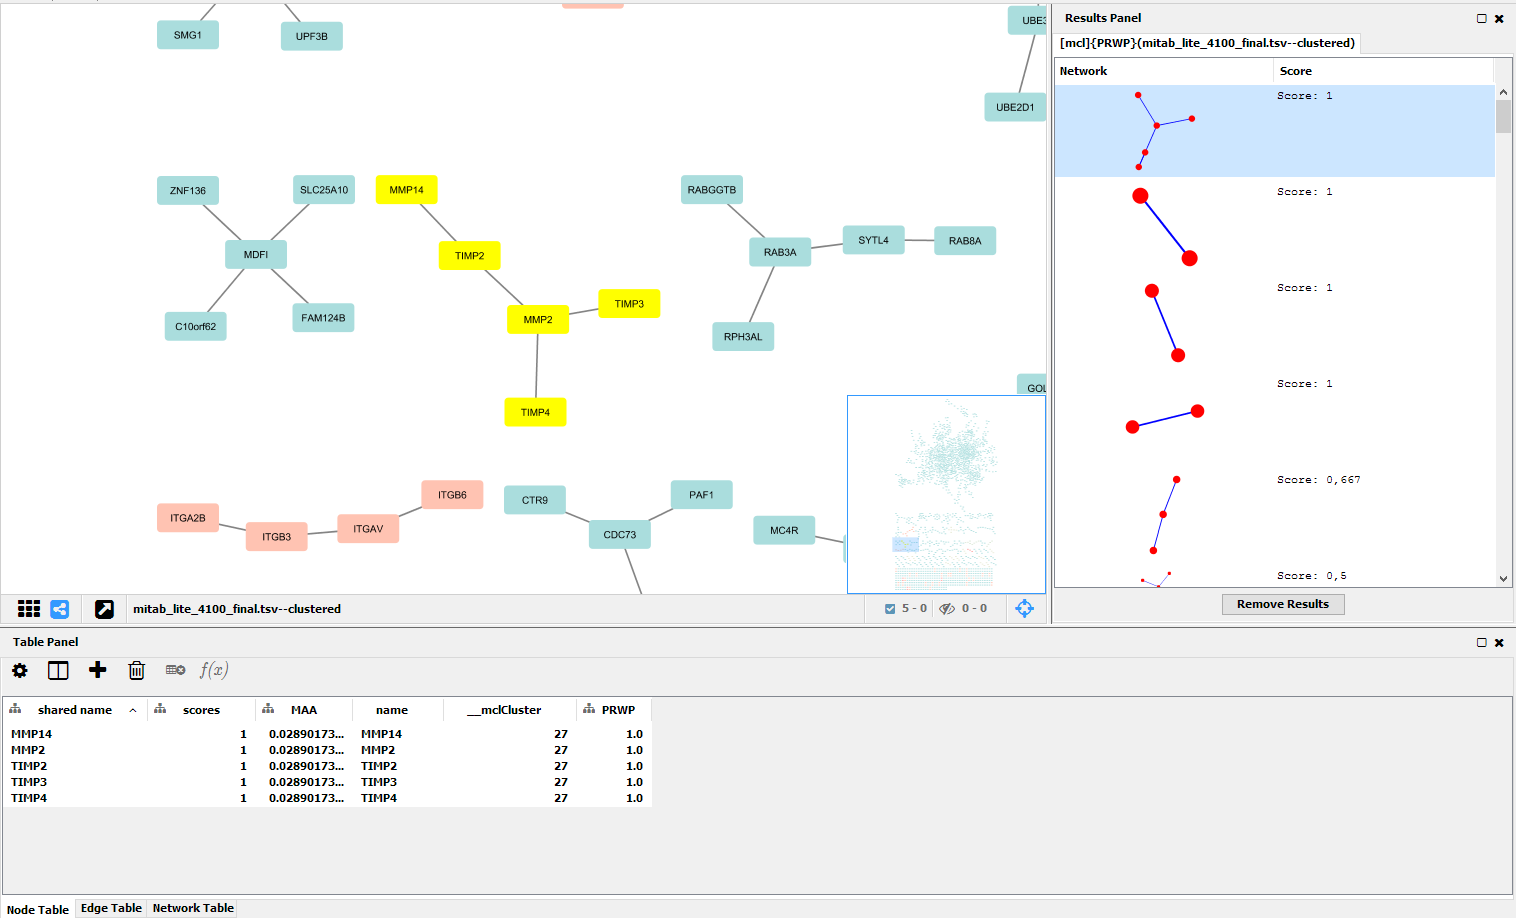
\includegraphics[width=15cm]{12-rank-selection}
    \caption{Change the color of the nodes in a cluster when the cluster is
    selected from the results panel}
    \label{fig:rank-selection}
\end{figure}

\section{Design}
The class relations in Ranklust's ranking algorithms and ranking results panel
are described below in simple UML diagrams. The goal of this design was to have
an implementation of the ranking algorithms and the panel as close to the
existing clustering algorithms and results panel. 

\begin{figure}[H]
    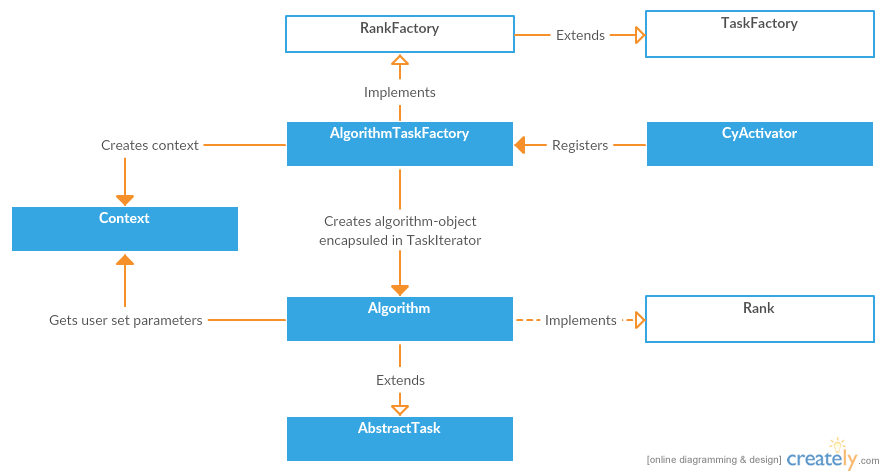
\includegraphics[width=\textwidth]{ranklust-algorithm}
    \caption{UML diagram for Ranklust's class relations for the ranking
    algorithms}
    \label{fig:rank-alg}
\end{figure}

The ranking algorithm relations (Figure: \ref{fig:rank-alg}) shows how the
classes are connected together and what they offer. The context is not
self-explanatory, but it has responsibility for the GUI component that
represents each specific ranking algorithm. Each algorithm in Ranklust has its
own instance of the following classes:

\begin{itemize}
    \item AlgorithmTaskFactory
    \item Context
    \item Algorithm
\end{itemize}

The rest of the classes are are not unique to any of the ranking algorithms.

\begin{figure}[H]
    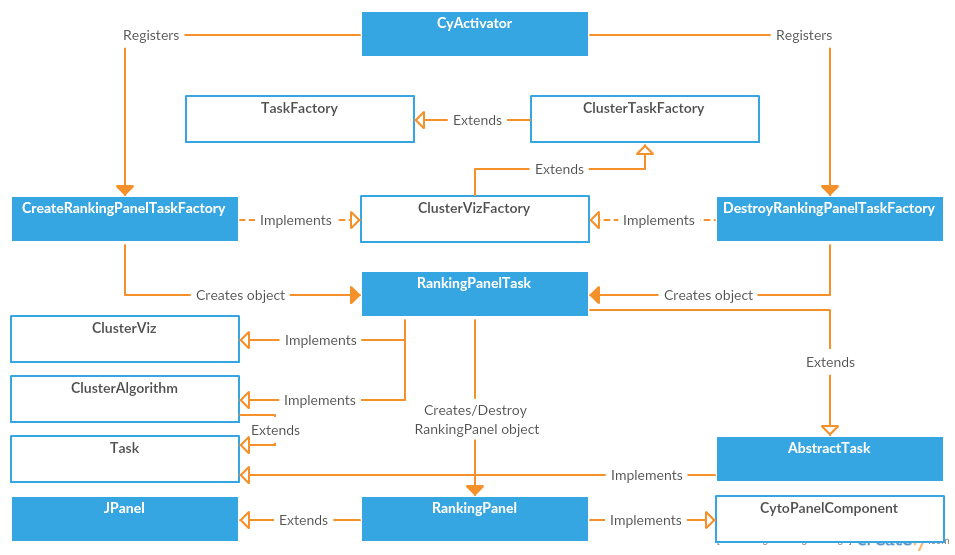
\includegraphics[width=\textwidth]{ranklust-panel}
    \caption{UML diagram for Ranklust's class relations for the ranking results
    panel}
    \label{fig:rank-panel}
\end{figure}

The ranking panel relations (Figure: \ref{fig:rank-panel}) shows how the classes
are connected to the ranking panel. The "Create" and "Destroy" task factories
exists to be able to destroy all of the panels ranking clusters, or to create
a new one. They are two separate classes to appear in the Cytoscape menu as two
separate options. Both of these two classes returns a RankingPanelTask object,
where the arguments sent to its class constructor defines whether if the task
should create or destroy a panel. An advantage to have two separate classes
responsible for creating or destroying a panel is the ability to make them
unavailable. For example, it is not possible for the user to select the "Destroy
All Cluster Results Panels" in the "clusterMaker Visualizations" menu, if no
ranking results panels exists.

\chapter{Prioritizing network biomarkers in prostate cancer through graph analysis}
\section{How the network was created}
After querying iRefWeb for the PPI-network with the query displayed earlier
(figure \ref{fig:irefweb}) the resulting network consisted of 109276 interactions.
After filtering the same network through the protein-to-gene mapping constructed
from HGNC, the final network consisted of 9500 nodes (genes) and 43706 edges
(interactions). At this point, all of the nodes and edges were undirected and
unweighted. Converting from proteins to genes ended up with a 60\% perturbation
of the network in the form of removed edges. Clustering the network resulted in
a further perturbation of 69.8\% of edge-removal when compared to the
HGNC-filtered network, 87.9\% when compared to the unfiltered iRefWeb network.

The creation of the \gls{golden} through combining DisGeNET and \gls{dragon}
resulted in a file with two columns. One representing a gene, the second one
representing the score of a gene, so a single row would contain a unique gene in
the list and the score it received.

\section{Which parameters for clustering was used and why}
Talking about \gls{mcl} results
\begin{table}[H]
    \centering
    \begin{tabular}{| l | p{2cm} | p{2cm} | p{2cm} | p{2cm} | p{2cm} | p{2.1cm} |}
        \hline
        \textbf{Inflation} & \textbf{Clusters} & \textbf{Avg.  cluster size} &
        \textbf{Max. cluster size} & \textbf{Min. cluster size} &
        \textbf{Modularity} \\
        \hline
        1.6 & 1068 & 8.88 & 968 & 2 & 0.367 \\
        1.8 & 1400 & 6.60 & 660 & 2 & 0.307 \\
        2.0 & 1599 & 5.68 & 405 & 2 & 0.269 \\
        2.5 & 2053 & 4.20 & 179 & 2 & 0.223 \\
        3.0 & 2210 & 3.75 & 122 & 2 & 0.199 \\
        \hline
    \end{tabular}
    \caption{MCL clustering parameter and statistic results}
    \label{tab:mcl-inflation}
\end{table}
The modularity of the clustered networks gives an indicator of how well the
process of creating the clusters went. Modularity is given as a score from 0 to
1. A score closer to 1 is more preferable, as this indicates that the clusters
created have a good degree of separation to the other clusters in the network.
The preferred score to end up with would be around 0.8, but in this network
there has been a good amount of perturbation through the protein-to-gene
process. Modularity is not the only indicator of how well a network was
clustered, hence the choice of not setting the inflation value in \gls{mcl} to
1.6, but rather 1.8. When a lower inflation value is set, \gls{mcl} does not
separate edges between nodes as vigorously and as a direct cause, inflation will
go up. Taking the other attributes in the table (table: \ref{tab:mcl-inflation}) into
consideration, 1.8 seemed like the best inflation value. An inflation value of
1.8 has also been proved to be good for large high-throughput constructed
protein-protein networks with a large amount of alterations\cite{mcl-inflation}.

The amount of iterations used for \gls{mcl} ended up being 200. It started out
at 1000, but the results converged somewhere between 170 and 200 iterations, so
it was decreased form 1000 to 200 to speed up the time used in the
\gls{pipeline}.

\section{Results from cross-validation and what they indicate}
\begin{sidewaysfigure}
    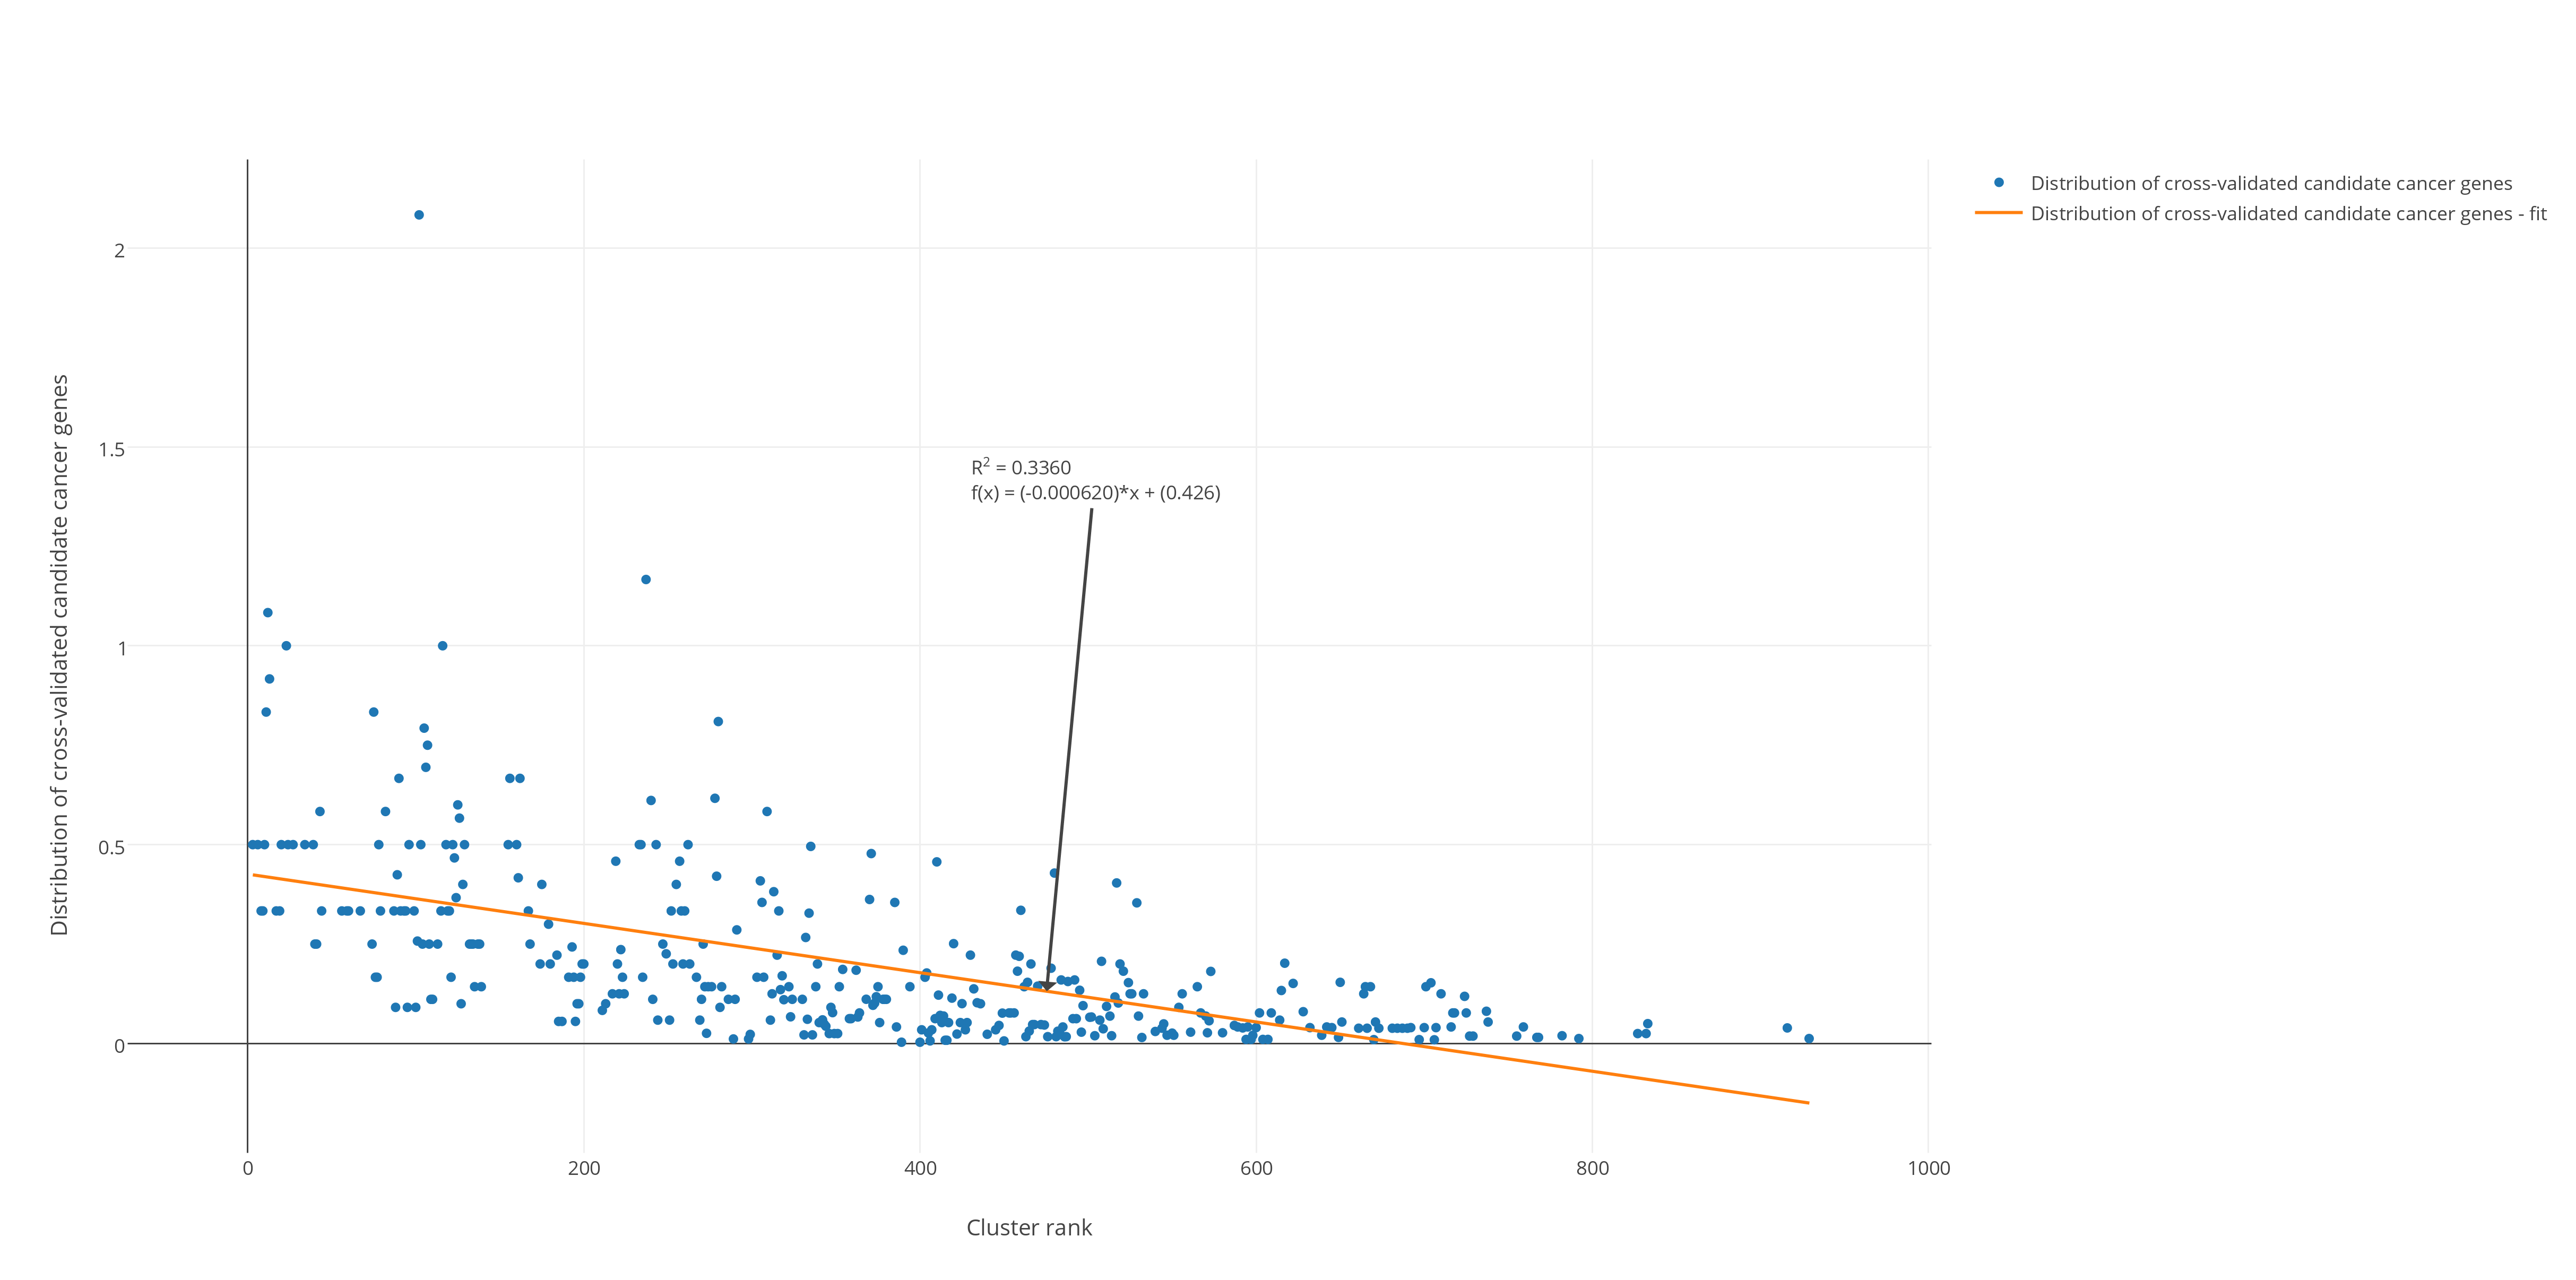
\includegraphics[scale=0.63]{cv_dist_total_filtered_prwp}
    \caption{Distribution of combined averages of genes, which had their scores
    \label{fig:irefweb-prwp}
    removed by cross-validation, ranked by PRWP}
\end{sidewaysfigure}

\begin{sidewaysfigure}
    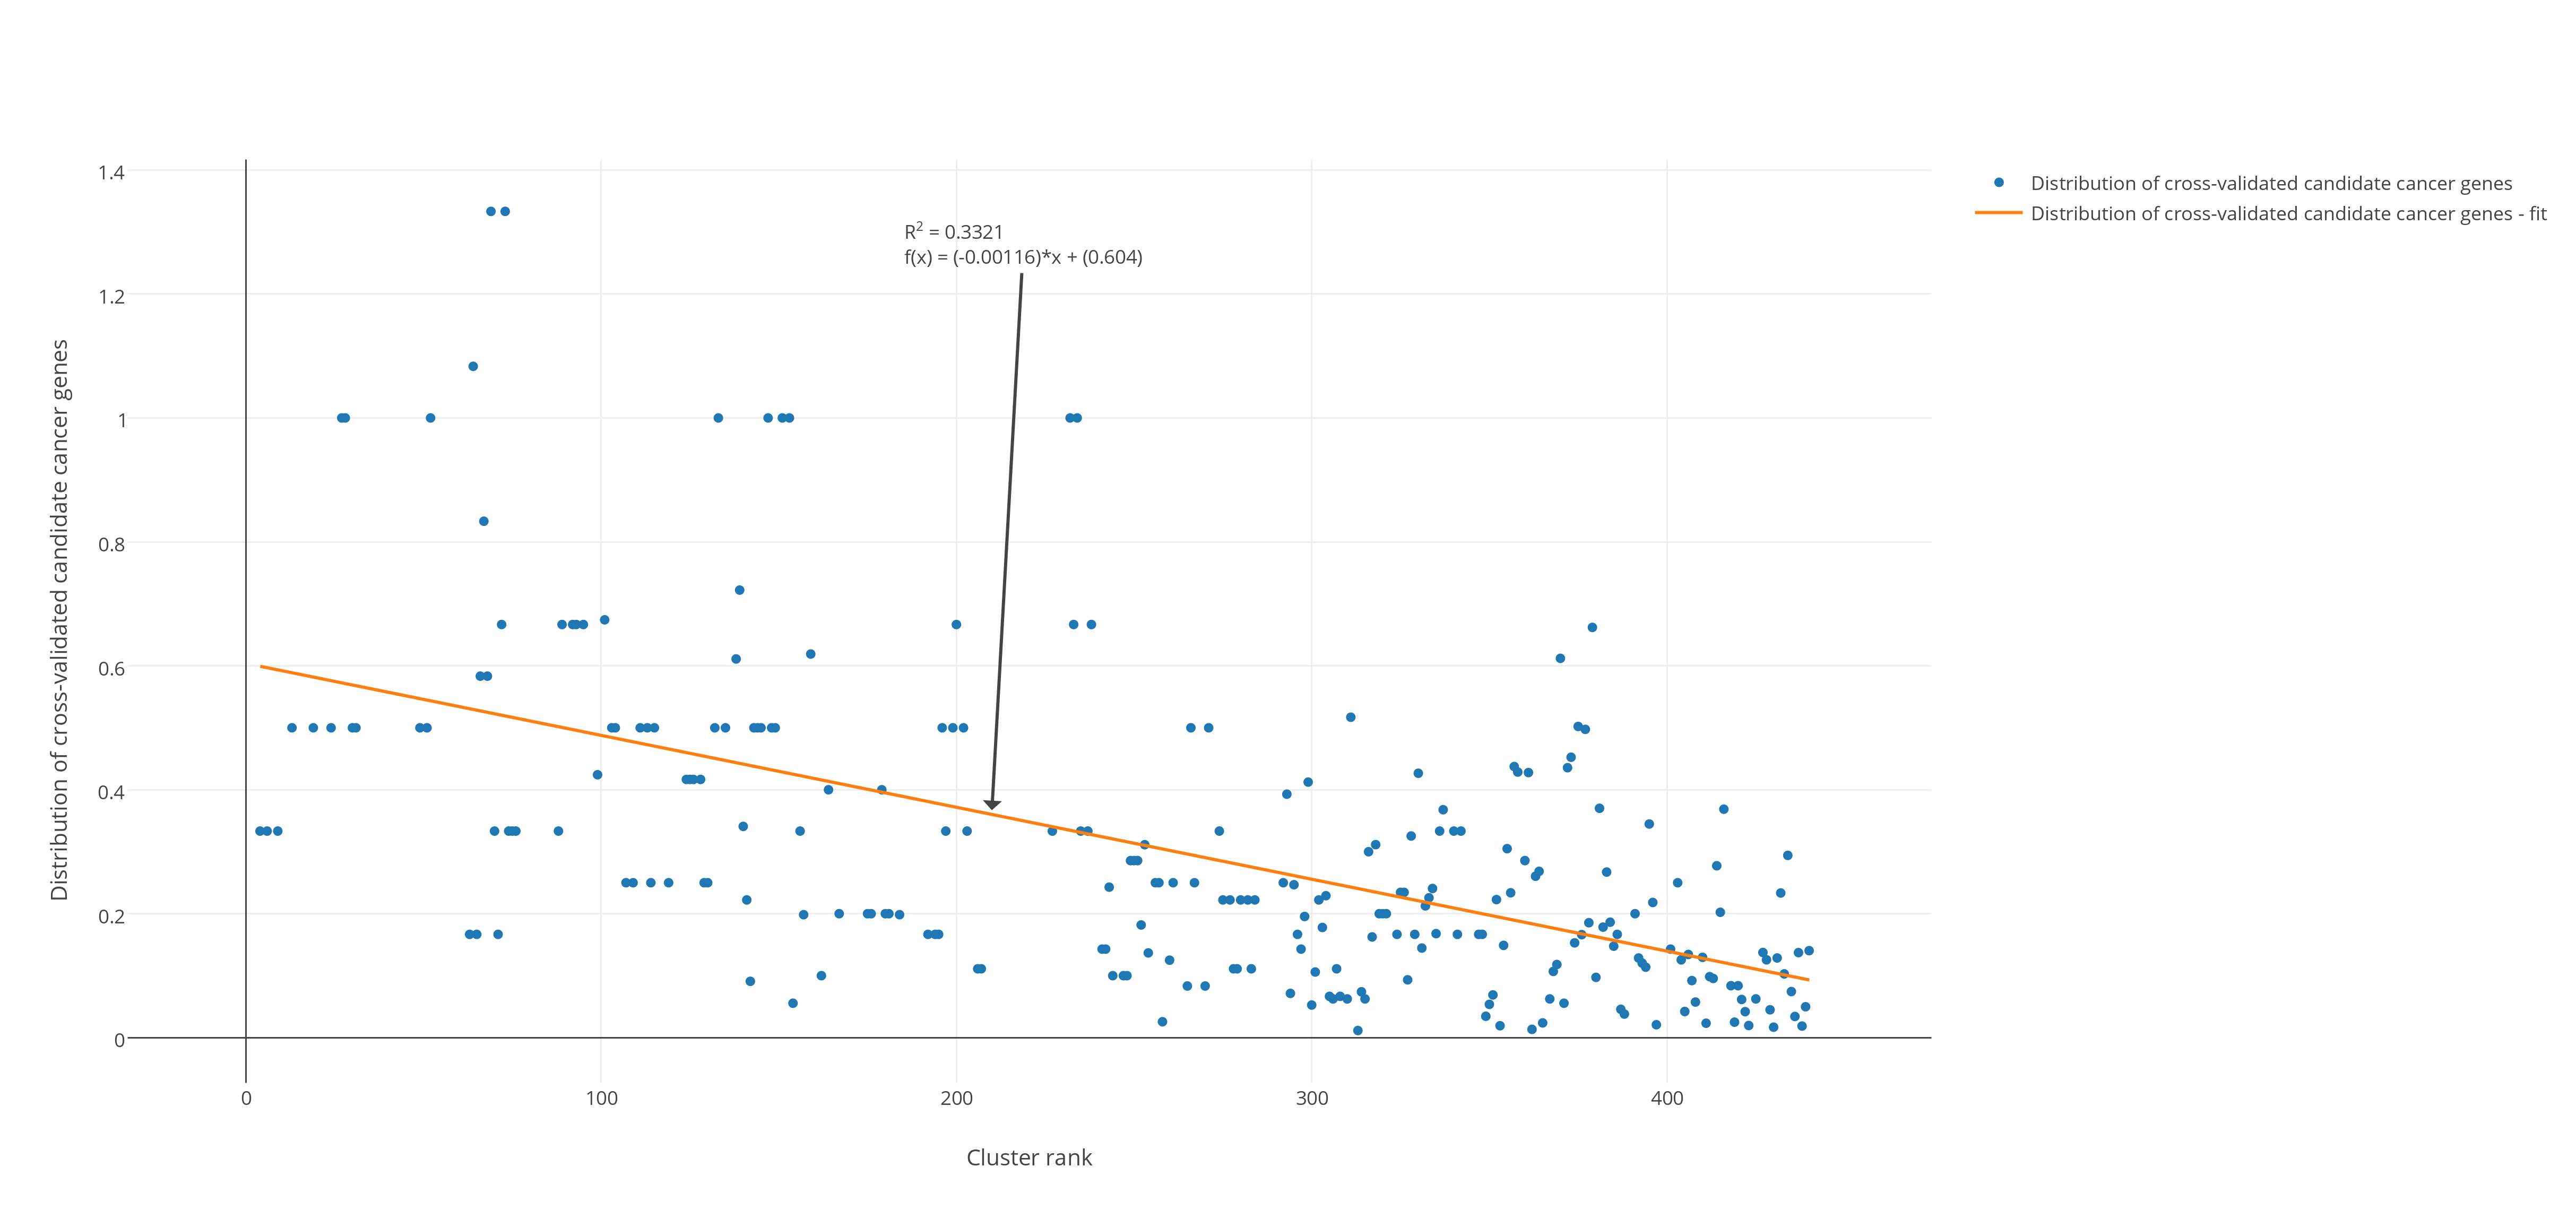
\includegraphics[scale=0.63]{cv_dist_total_filtered_maa}
    \caption{Distribution of combined averages of genes, which had their scores
    \label{fig:irefweb-maa}
    removed by cross-validation, ranked by MAA}
\end{sidewaysfigure}

The plots in figure \ref{fig:irefweb-prwp} and figure \ref{fig:irefweb-maa} is
developed from the 10 random cross-validation runs ranked with \gls{prwp} and
\gls{maa}. The x-axis represents the cluster ranks which is represented as
a blue dot in the scatter plot. Each rank consists of a single cluster which has
an arbitrary number of genes above 1. The y-axis represents a result from two
steps. The first step was to go through each of the
10 cross-validated results from ranking the iRefWeb network with \gls{prwp} and
\gls{maa}. In each of the cross-validated results an average was calculated for
each cluster. The average was calculated from dividing the number of genes, that
had their prior score removed as a result of the cross-validation, by the total
number of genes in the cluster. Each cluster would at this point have an average
representing the average of cross-validated genes in a cluster. The second step
completes the values for the y-axis in the plot and represents the score in
a cluster when additively combining the averages from each of the 10
cross-validated results that was found by \gls{prwp} and \gls{maa}. To filter
out the uninteresting results, all zero values on the y-axis was removed.

The analysis of which clusters contained the largest combined average of genes,
which had their prior score removed by cross-validation, shows that the topmost
ranked clusters had the highest combined average. This information indicates
that ranking clusters with \gls{prwp} and \gls{maa} have a tendency towards
ranking the larger part of the population of prostate cancer biomarkers at the
top of the cluster ranks, and the lower at the bottom.

Executing a cross-validation on the iRefWeb with \gls{prwp} and \gls{maa}
rankings had two purposes. The first being to prove the fact that every gene
that had its prior score removed by the cross-validation, should be found in the
results of the cluster ranking and identified as candidate biomarkers. The
second, to prove that the distribution of the combined average in the clusters
should correlate to the rank they obtained through Ranklust's use of \gls{prwp}
and \gls{maa}.

\subsection{Differences between ranking with PRWP and MAA}
There is clearly a trend in both \gls{prwp} and \gls{maa}. The difference
between them being mainly the number of clusters ranked and the coupling of
values around the linear regression fit. It is important to point out that this
is just a result over the distribution of candidate cancer genes at certain
ranks. Where the clusters resides in the rankings may be very different between
the \gls{prwp} and \gls{maa}.

The values in \gls{prwp} have a tighter coupling, in other words, the distance
the coordinates have in the scatter plot deviate less from the fit than the ones
in the \gls{maa} plot. The difference is not huge, as the coefficient of
determination indicates 0.336 in \gls{prwp} against 0.332 in \gls{maa}. Both
ranking algorithms achieves a descending distribution of cross-validated genes
from the topmost to the lowest ranked cluster. Though, when comparing the
cross-validation results between \gls{prwp} and \gls{maa}, \gls{prwp} comes out
ahead by a margin in \gls{rsquared} value.

\chapter{Benchmarking Ranklust against text mined, curated knowledge and experimental test data}
\section{Retrieving the test data from the DISEASE database}
Benchmarking Ranklust is done against three resources of data from a single
database called DISEASE\cite{jensen}. This database can be queried for diseases
or genes. The query in this database was limited to searching for a single
disease or gene name. No API was found to access the database directly, so to
retrieve the gene names related to prostate cancer, whole files was downloaded.
There were three files, one for each type of research put into retrieving the
data: text mined, manually curated knowledge and experimental data. Each of
these files was filled with genes and their relation to different diseases, so
they had to be filtered to only contain genes with information about prostate
cancer. This was done by only using genes that contained "prostate cancer" in
the column indicating which disease the specific gene was related to.

The plots representing values in clusters from each of these three files have
split each cluster in two parts, blue and orange. The blue dots in the scatter
plot represents the genes in a cluster that has prior scores. The orange dots in
the scatter plot represent genes in the same cluster as the blue ones in terms
of which rank they are in based on the x-axis, but they do not have prior
scores. The blue dots are also mentioned as prostate cancer genes and orange
dots as prostate candidate cancer genes, because they have no score, but they
are in some cases related to other prostate cancer genes to such a degree that
they are susceptible to be candidate cancer biomarkers for prostate cancer. As
with the cross-validation plots, the zero values in the plots have been removed.

\section{Z-scores for text mined genes in clusters}
\begin{sidewaysfigure}
    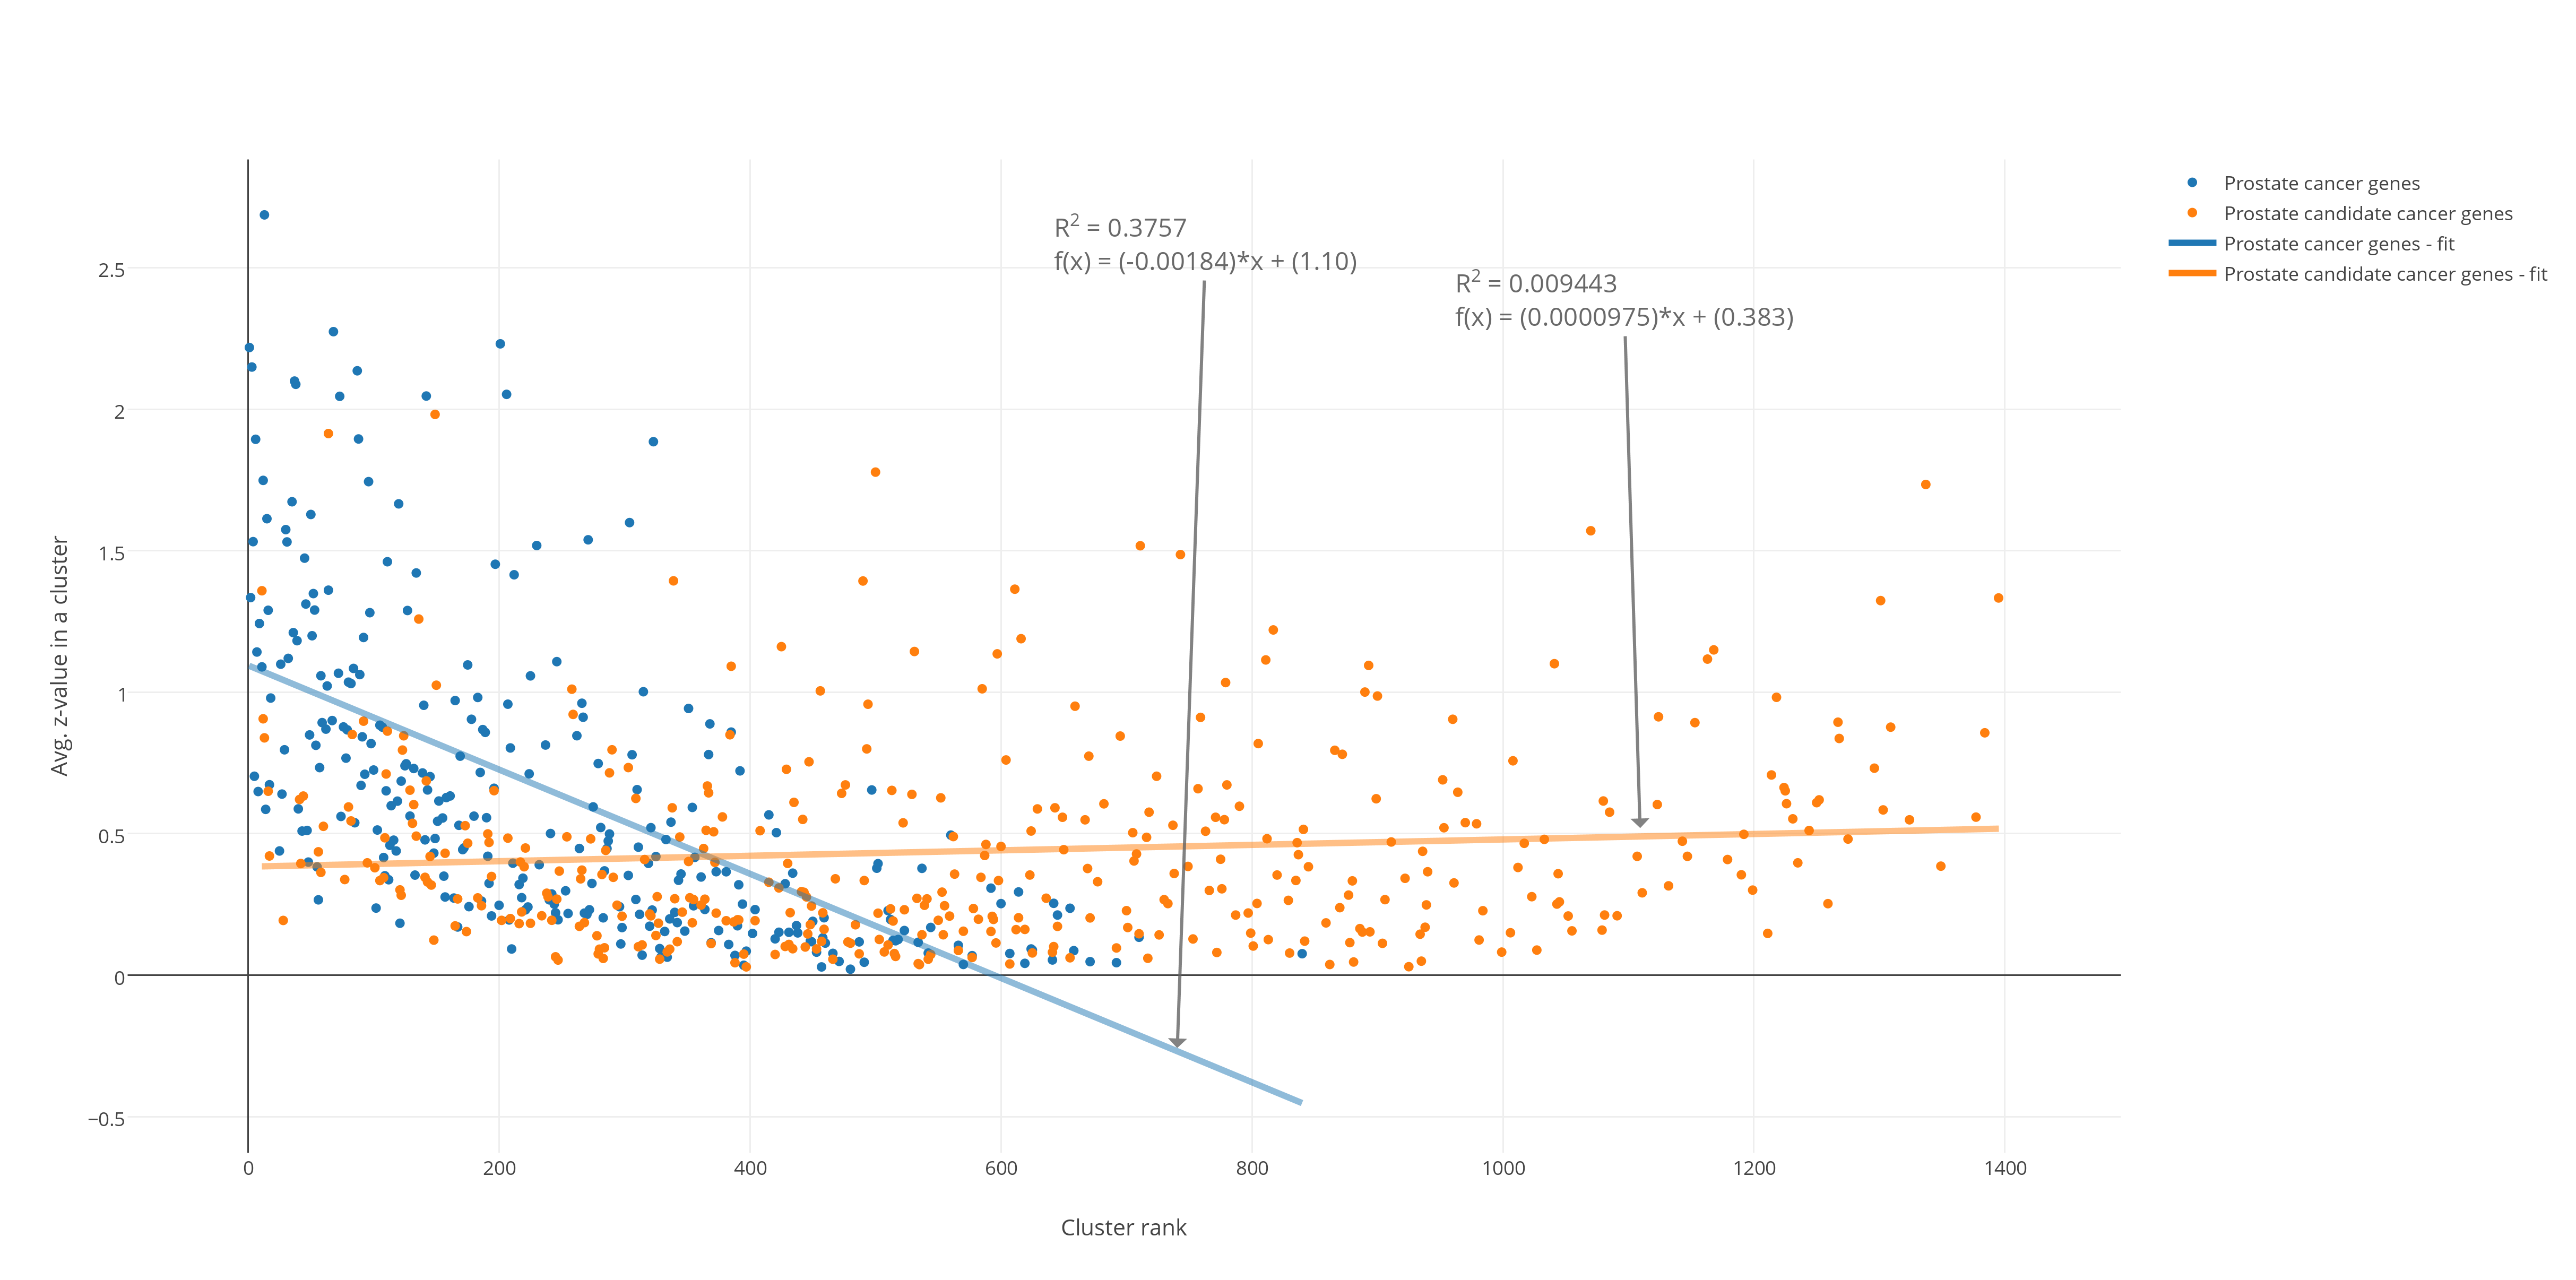
\includegraphics[scale=0.63]{prwp_txt_split}
    \caption{Average z-score in a cluster ranked by PRWP}
    \label{fig:txt-iref-prwp}
\end{sidewaysfigure}
\begin{sidewaysfigure}
    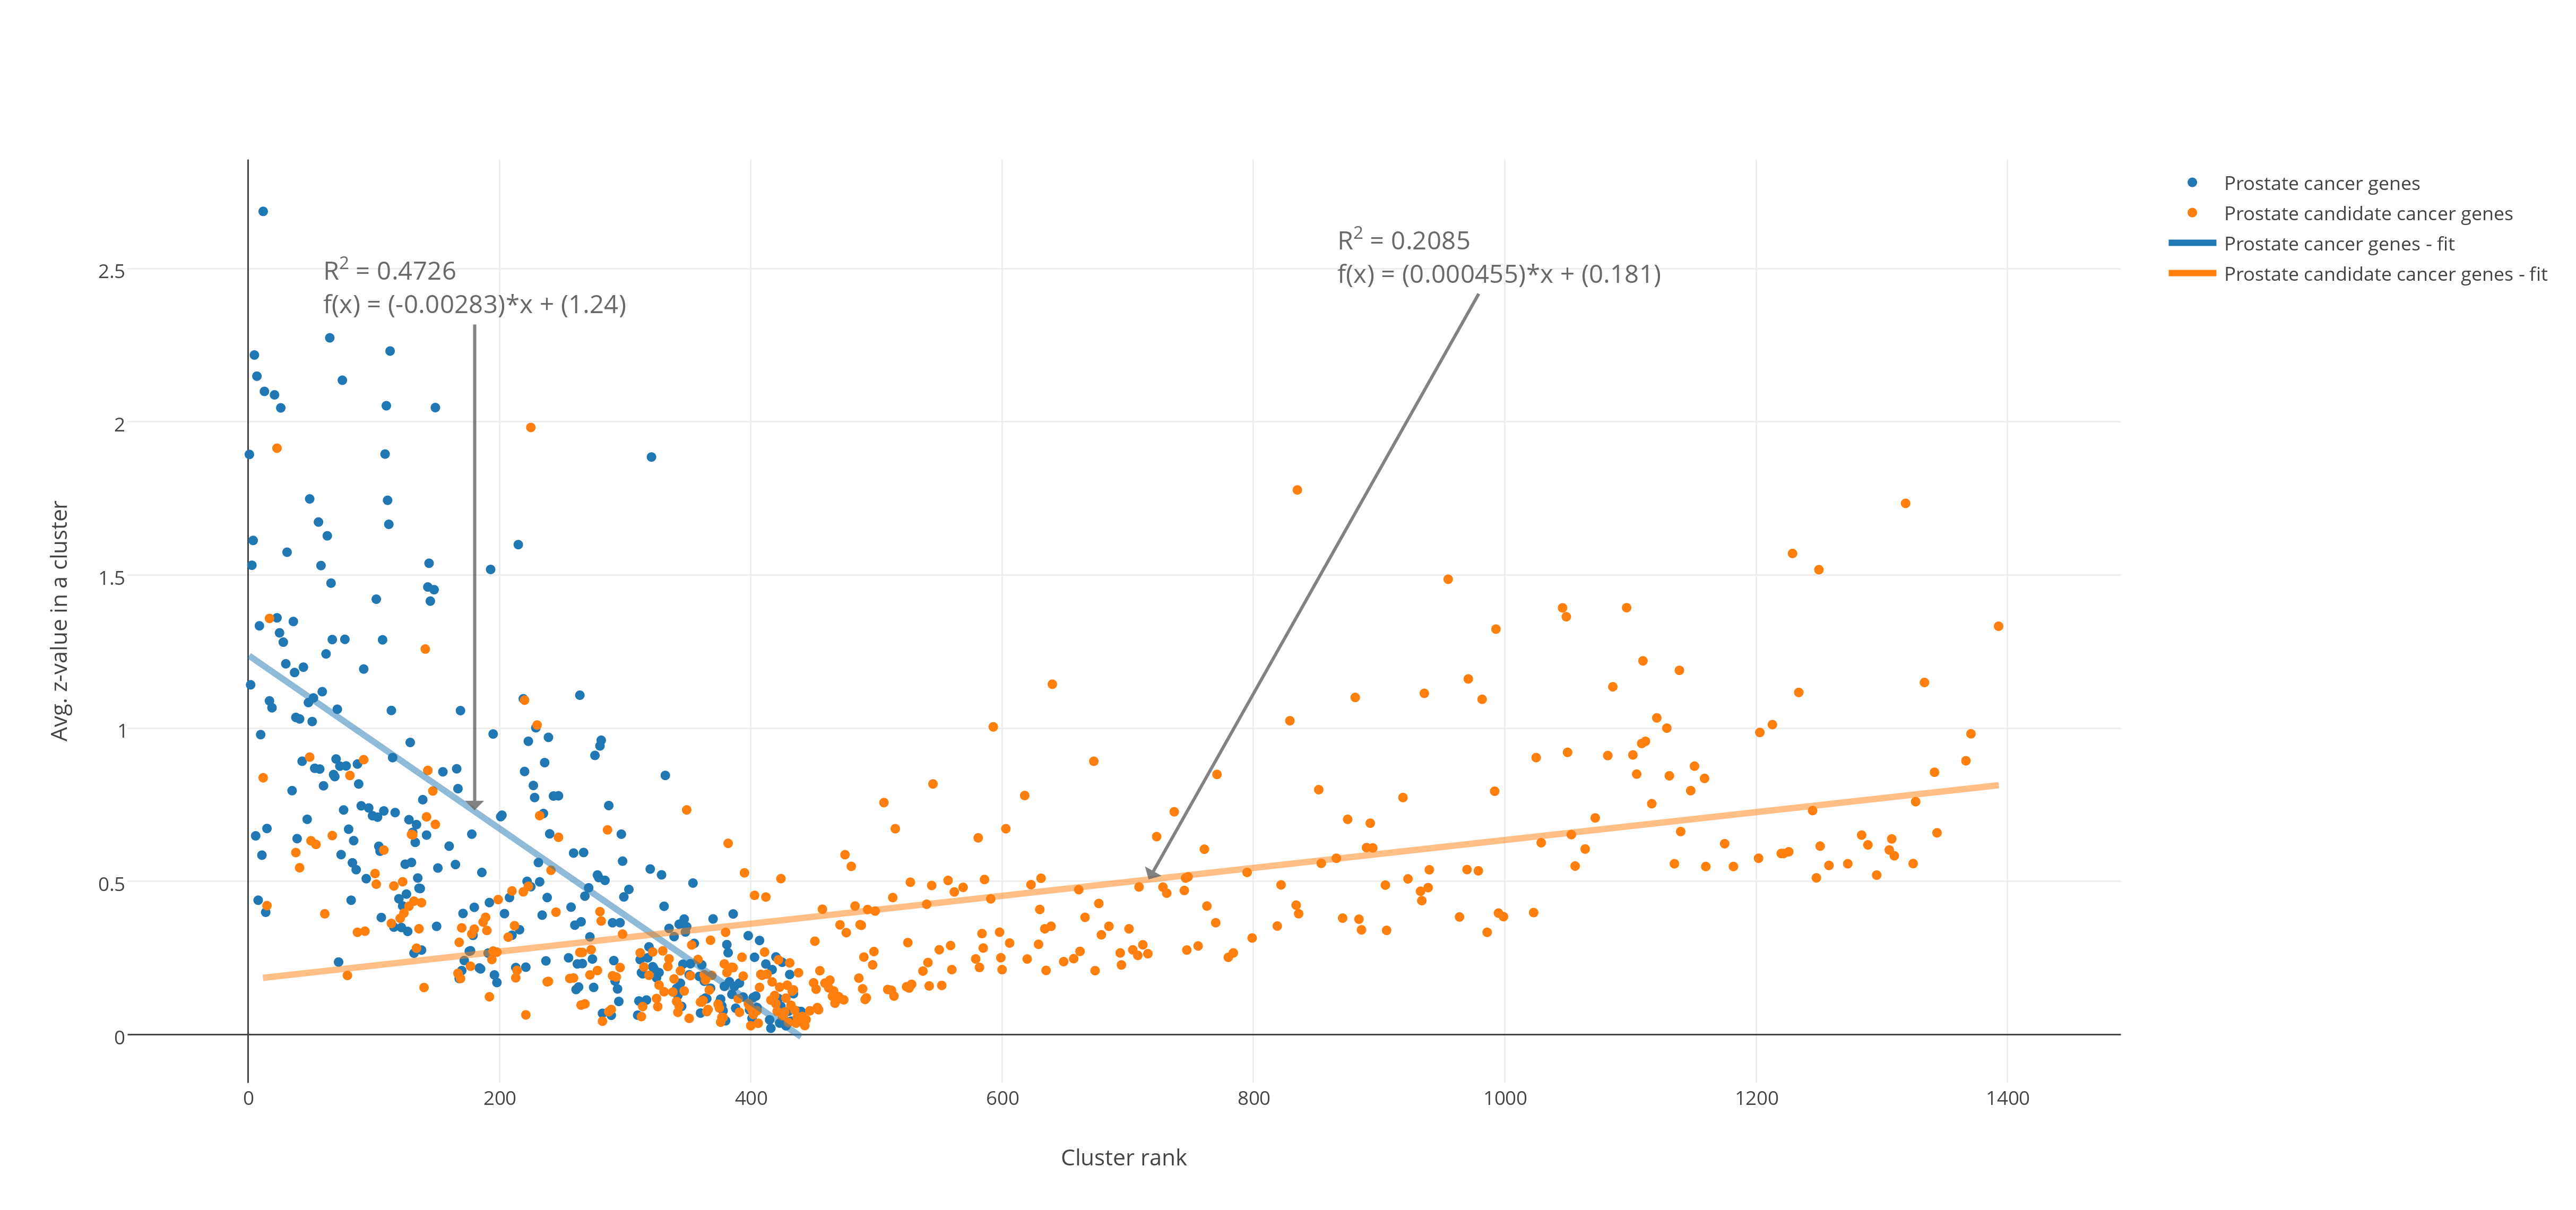
\includegraphics[scale=0.63]{maa_txt_split}
    \caption{Average z-score in a cluster ranked by MAA}
    \label{fig:txt-iref-maa}
\end{sidewaysfigure}

The text mined scores are represented by a z-score. The z-score to a gene in the
text mined data from the DISEASE database is a developed from a co-occurrence
score, which increased when a gene and a disease was mentioned together, but
also decreased when they were mentioned with multiple other genes or diseases.
This co-occurrence score was later converted to z-scores to be more robust to
changes to the size of the text corpus in the DISEASE database\cite{jensen}.
This results in the average z-score to a cluster, which is based on the average
z-score of each gene in a cluster, to be a benchmark as to how high the cluster
should be ranked in terms of being a relevant network biomarker for prostate
cancer.

Since the plots have split each cluster into two parts, the cluster part of
genes with priors and the ones without priors, the expected outcome, should the
ranking algorithms perform as expected, would be to have the blue dots
descending and the orange dots ascending, when looking at a linear regression
fit going from the topmost ranked cluster to the lowest.

\subsection{PRWP benchmarked with text mined genes}
For \gls{prwp} (figure: \ref{fig:txt-iref-prwp}), the prostate cancer candidate genes is
descending in z-values from the topmost ranked cluster to the lowest, which is
contributing to showing \gls{prwp}'s suitability for ranking clusters as
candidate biomarkers.

The prostate candidate cancer biomarkers are ascending in z-value from the
topmost to the lowest ranked cluster. High z-values could contribute to the fact
that ranklust has found actual prostate candidate cancer biomarkers. However,
a low z-values does not contradict it. The only fact to deduce from low z-values
is that they have not been examinated to the degree that they are not mentioned
as a single gene related to prostate cancer in scientific papers.

\subsection{MAA benchmarked with text mined genes}
For \gls{maa} (figure: \ref{fig:txt-iref-maa}), the prostate cancer genes have the same
distinct descension in z-values from the topmost to the lowest cluster ranks.
The difference from \gls{prwp} to \gls{maa} being that \gls{maa} has a more
distinct ascending linear regression fit for the z-values in the prostate
candidate cancer genes.

\subsection{Conclusion of benchmarking through text mined genes}
This demonstrates the main difference between \gls{prwp} and \gls{maa}.
\gls{prwp} takes network structure into comparison as well as the prior scores,
so it will rank genes without priors higher than \gls{maa}. \gls{maa} focuses
purely on the prior scores, and so the network structure of protein complexes
are being completely ignored.

\section{Manually knowledge curated genes in a cluster}
\begin{sidewaysfigure}
    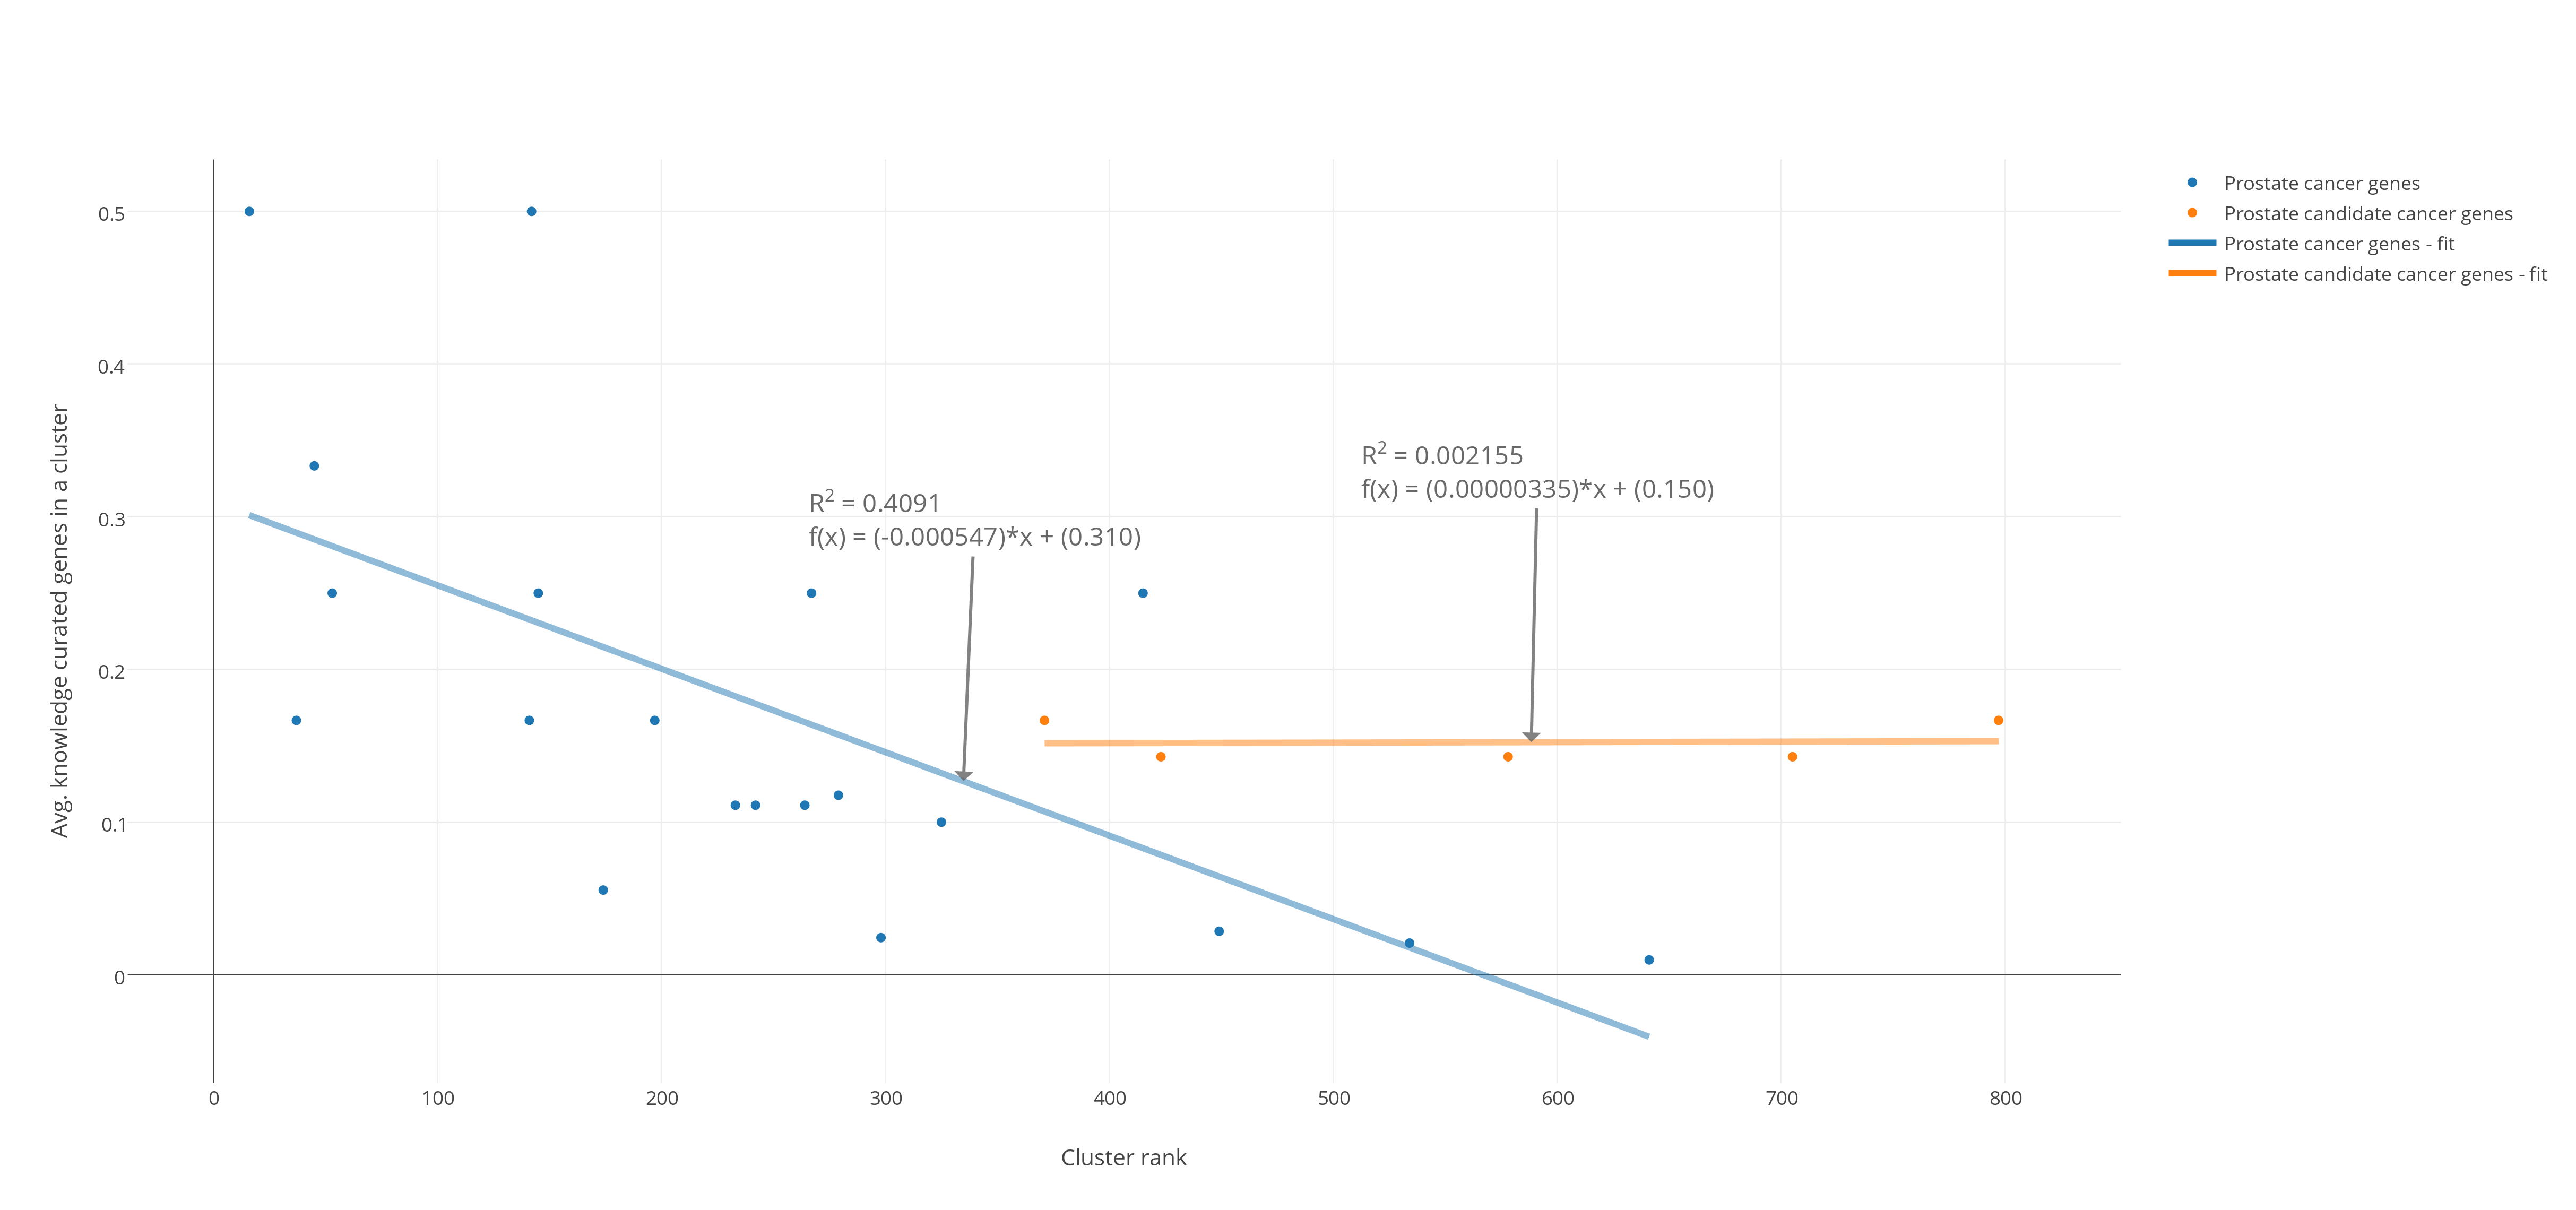
\includegraphics[scale=0.63]{prwp_know_split}
    \caption{Average distribution of curated knowledge mined genes in clusters
    ranked by PRWP.}
    \label{fig:know-iref-prwp}
\end{sidewaysfigure}

\begin{sidewaysfigure}
    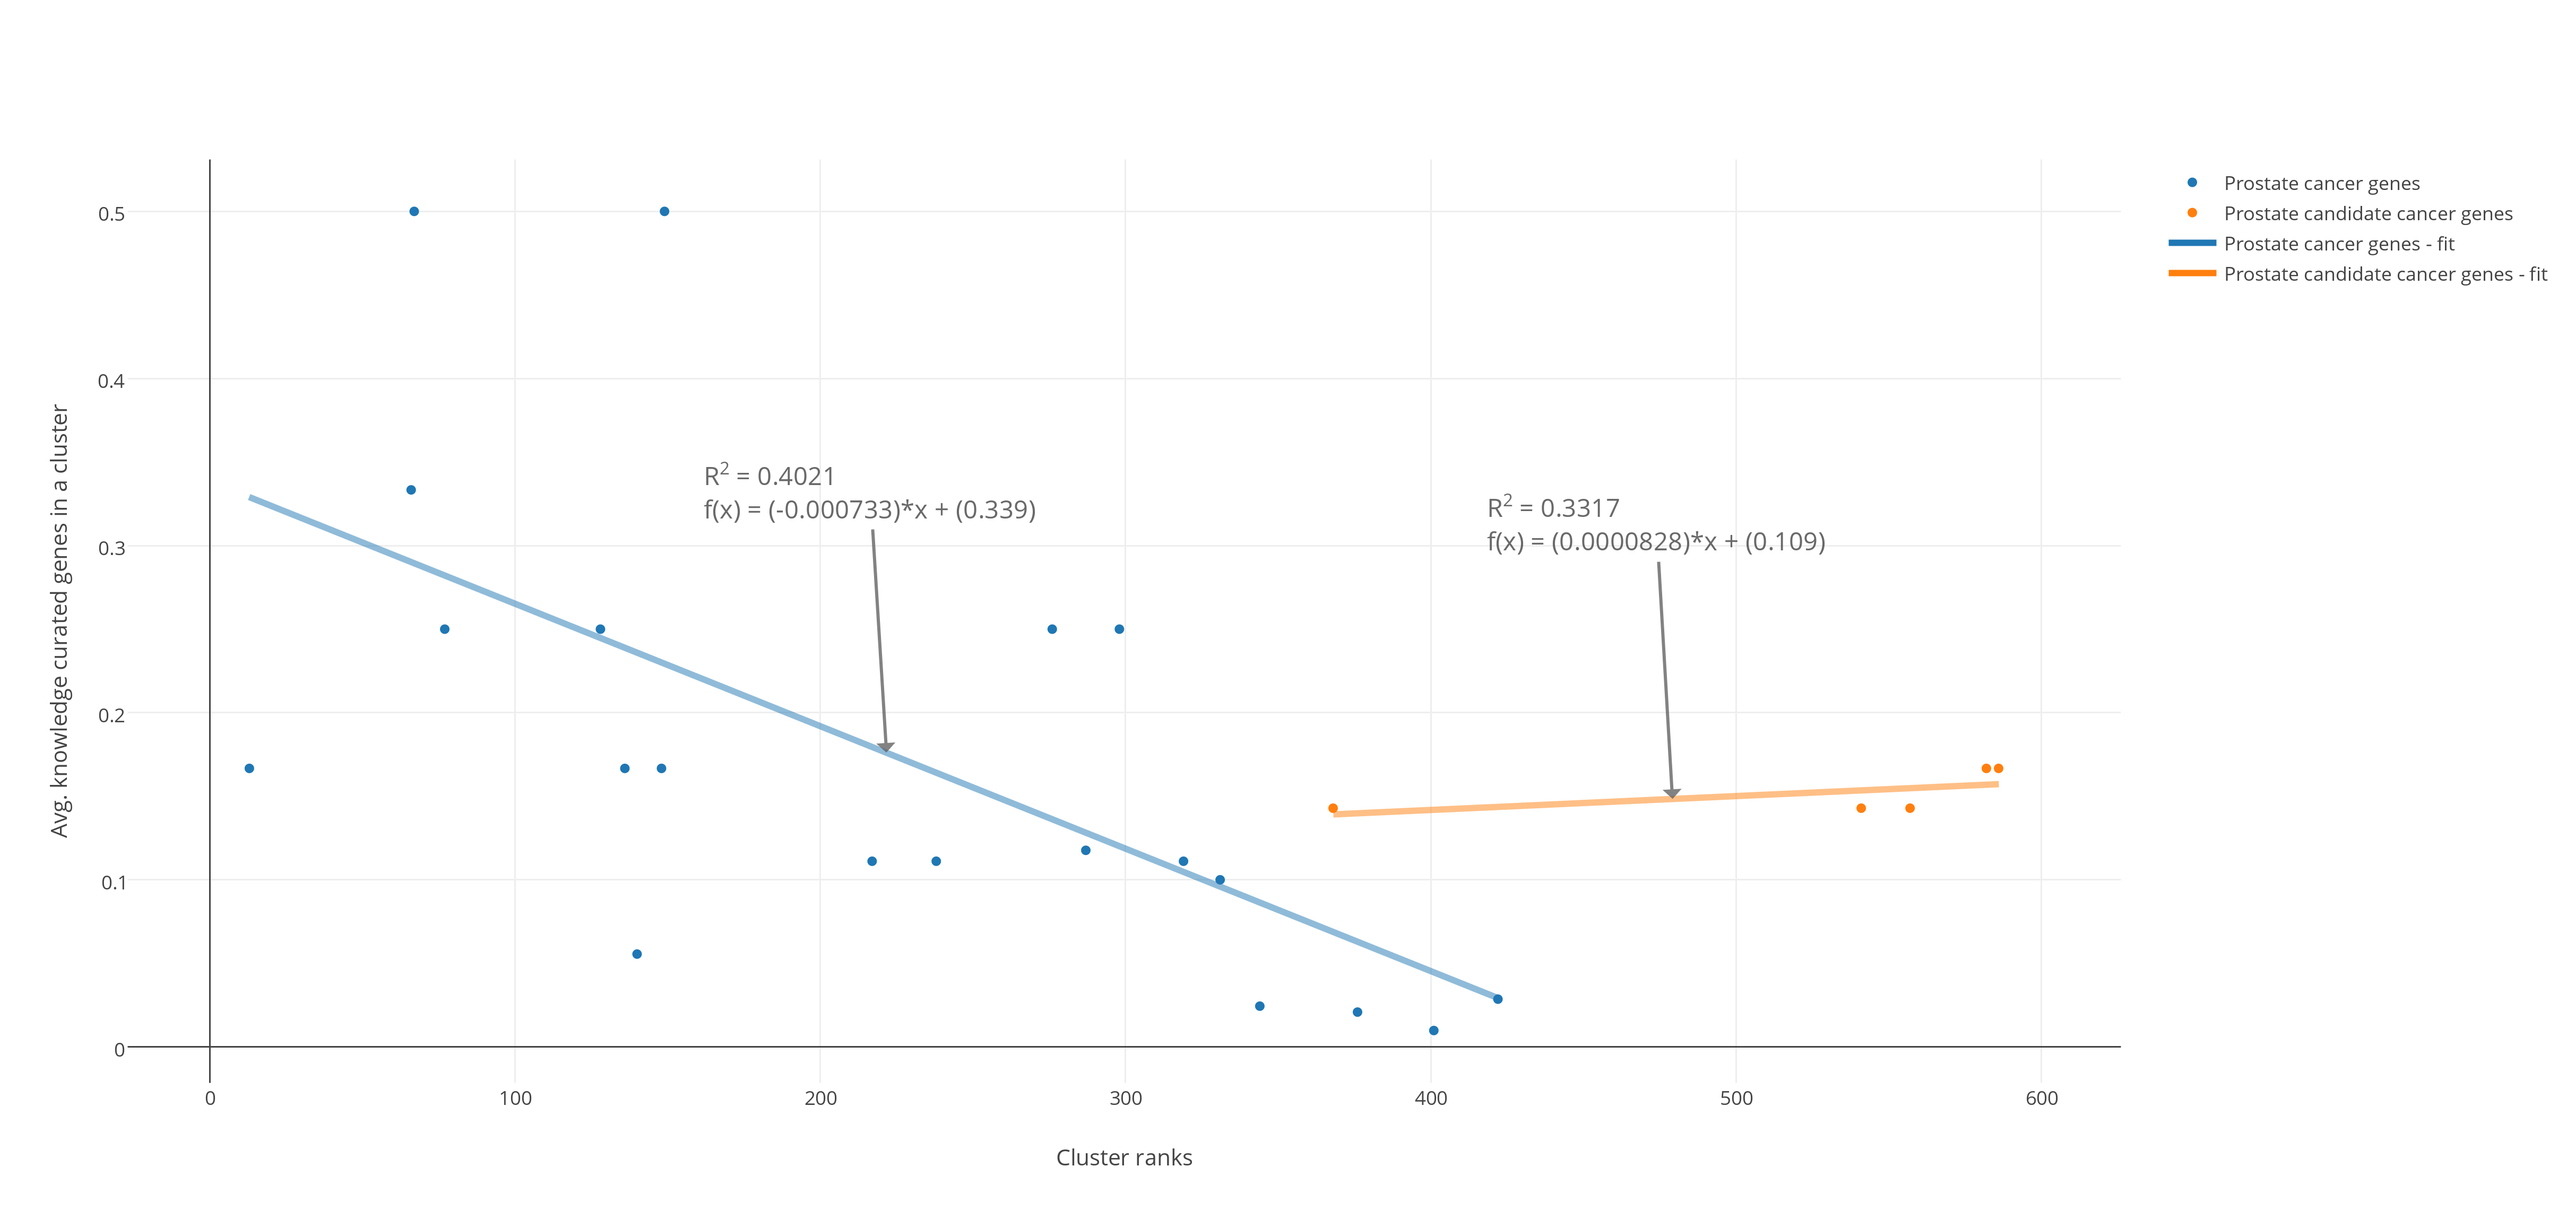
\includegraphics[scale=0.63]{maa_know_split}
    \caption{Average distribution of curated knowledge mined genes in clusters
    ranked by MAA.}
    \label{fig:know-iref-maa}
\end{sidewaysfigure}

This data had no score except for a confidence score in the \gls{jensen}
database. Every gene in the manually knowledge curated file had a confidence
score of 5 stars, due to being manually curated by researchers\cite{jensen}.
Therefore, the average number of genes in a cluster would receive a knowledge
score based on if the gene occurs in the knowledge curated part of the
\gls{jensen} database or not. So the knowledge curated data is only based on
occurrence, and not a specific value, in contrast to the text mined and
experimentally mined genes in the database. The clusters are split two-ways, in
a similar way that the benchmark with the text mined genes was, blue for genes
in the cluster which have priors and orange for the genes that do not have prior
scores.

Another trait the knowledge curated data possesses is the amount entries in the
\gls{jensen} database that has. Text mined data can be seen as the
high-throughput technology of retrieving relevant data from papers, while the
knowledge curated data is manually curated knowledge by researchers. This is why
the amount of entries for knowledge curated data is so sparse when compared to
text mined data.

For the manually knowledge curated genes to indicate valuable rankings of the
clusters, the genes with prior scores should have a descending trend from the
topmost ranked cluster to the lowest. If the genes without prior scores, have
a clear ascending trend from the topmost to the lowest ranked cluster, it would
have been a direct contradiction to the fact that the ranking algorithms should
be able to rank genes without prior scores in a reasonable way if they are
related to genes with priors. A higher frequency of manually knowledge curated
genes would increase the validity of these trends, should they occur,
especially if they are subtle.

\subsection{PRWP benchmarked by manually knowledge curated genes}
For \gls{prwp} (figure: \ref{fig:know-iref-prwp}), the genes with prior scores in
a cluster have a clear descending trend from the topmost to the lowest ranked
cluster. This builds up under the validitiy of \gls{prwp} being able to rank
prior scored genes correctly. The genes without prior scores in a cluster does
ascend to a low degree and the \gls{rsquared} for the fit that has this
ascending trend is not deemed as a good fit for the scores, at a \gls{rsquared}
value of only 0.002.

\subsection{MAA benchmarked by manually knowledge curated genes}
For \gls{maa} (figure: \ref{fig:know-iref-maa}), the genes with prior scores in a
cluster have the same trend as in \gls{prwp}. For the genes without prior scores
in a cluster, the trend also is the same as in \gls{prwp}, but to a higher
degree. The fit for the ascending average in manually knowledge curated genes in
a cluster, for the genes in the cluster without prior scores is an
\gls{rsquared} value of 0.33, which is considerably higher than the ascending
value for \gls{prwp}.

\subsection{Conclusion of benchmarking through manually knowledge curated genes}
Benchmarking \gls{maa} with manually knowledge curated gene test data has
uncovered its weakness of ranking prostate candidate cancer genes correctly.
\gls{prwp} had the same trend, but the fit was not very accurate and the trend
was negligible. Though, with such a small sample size of manually knowledge
curated genes when compared to text mined genes, \gls{maa} is excluded as
a viable ranking algorithm for prioritizing network biomarkers in prostate
cancer.

\section{Experimental genes distribution of p-values in genes}
\begin{sidewaysfigure}
    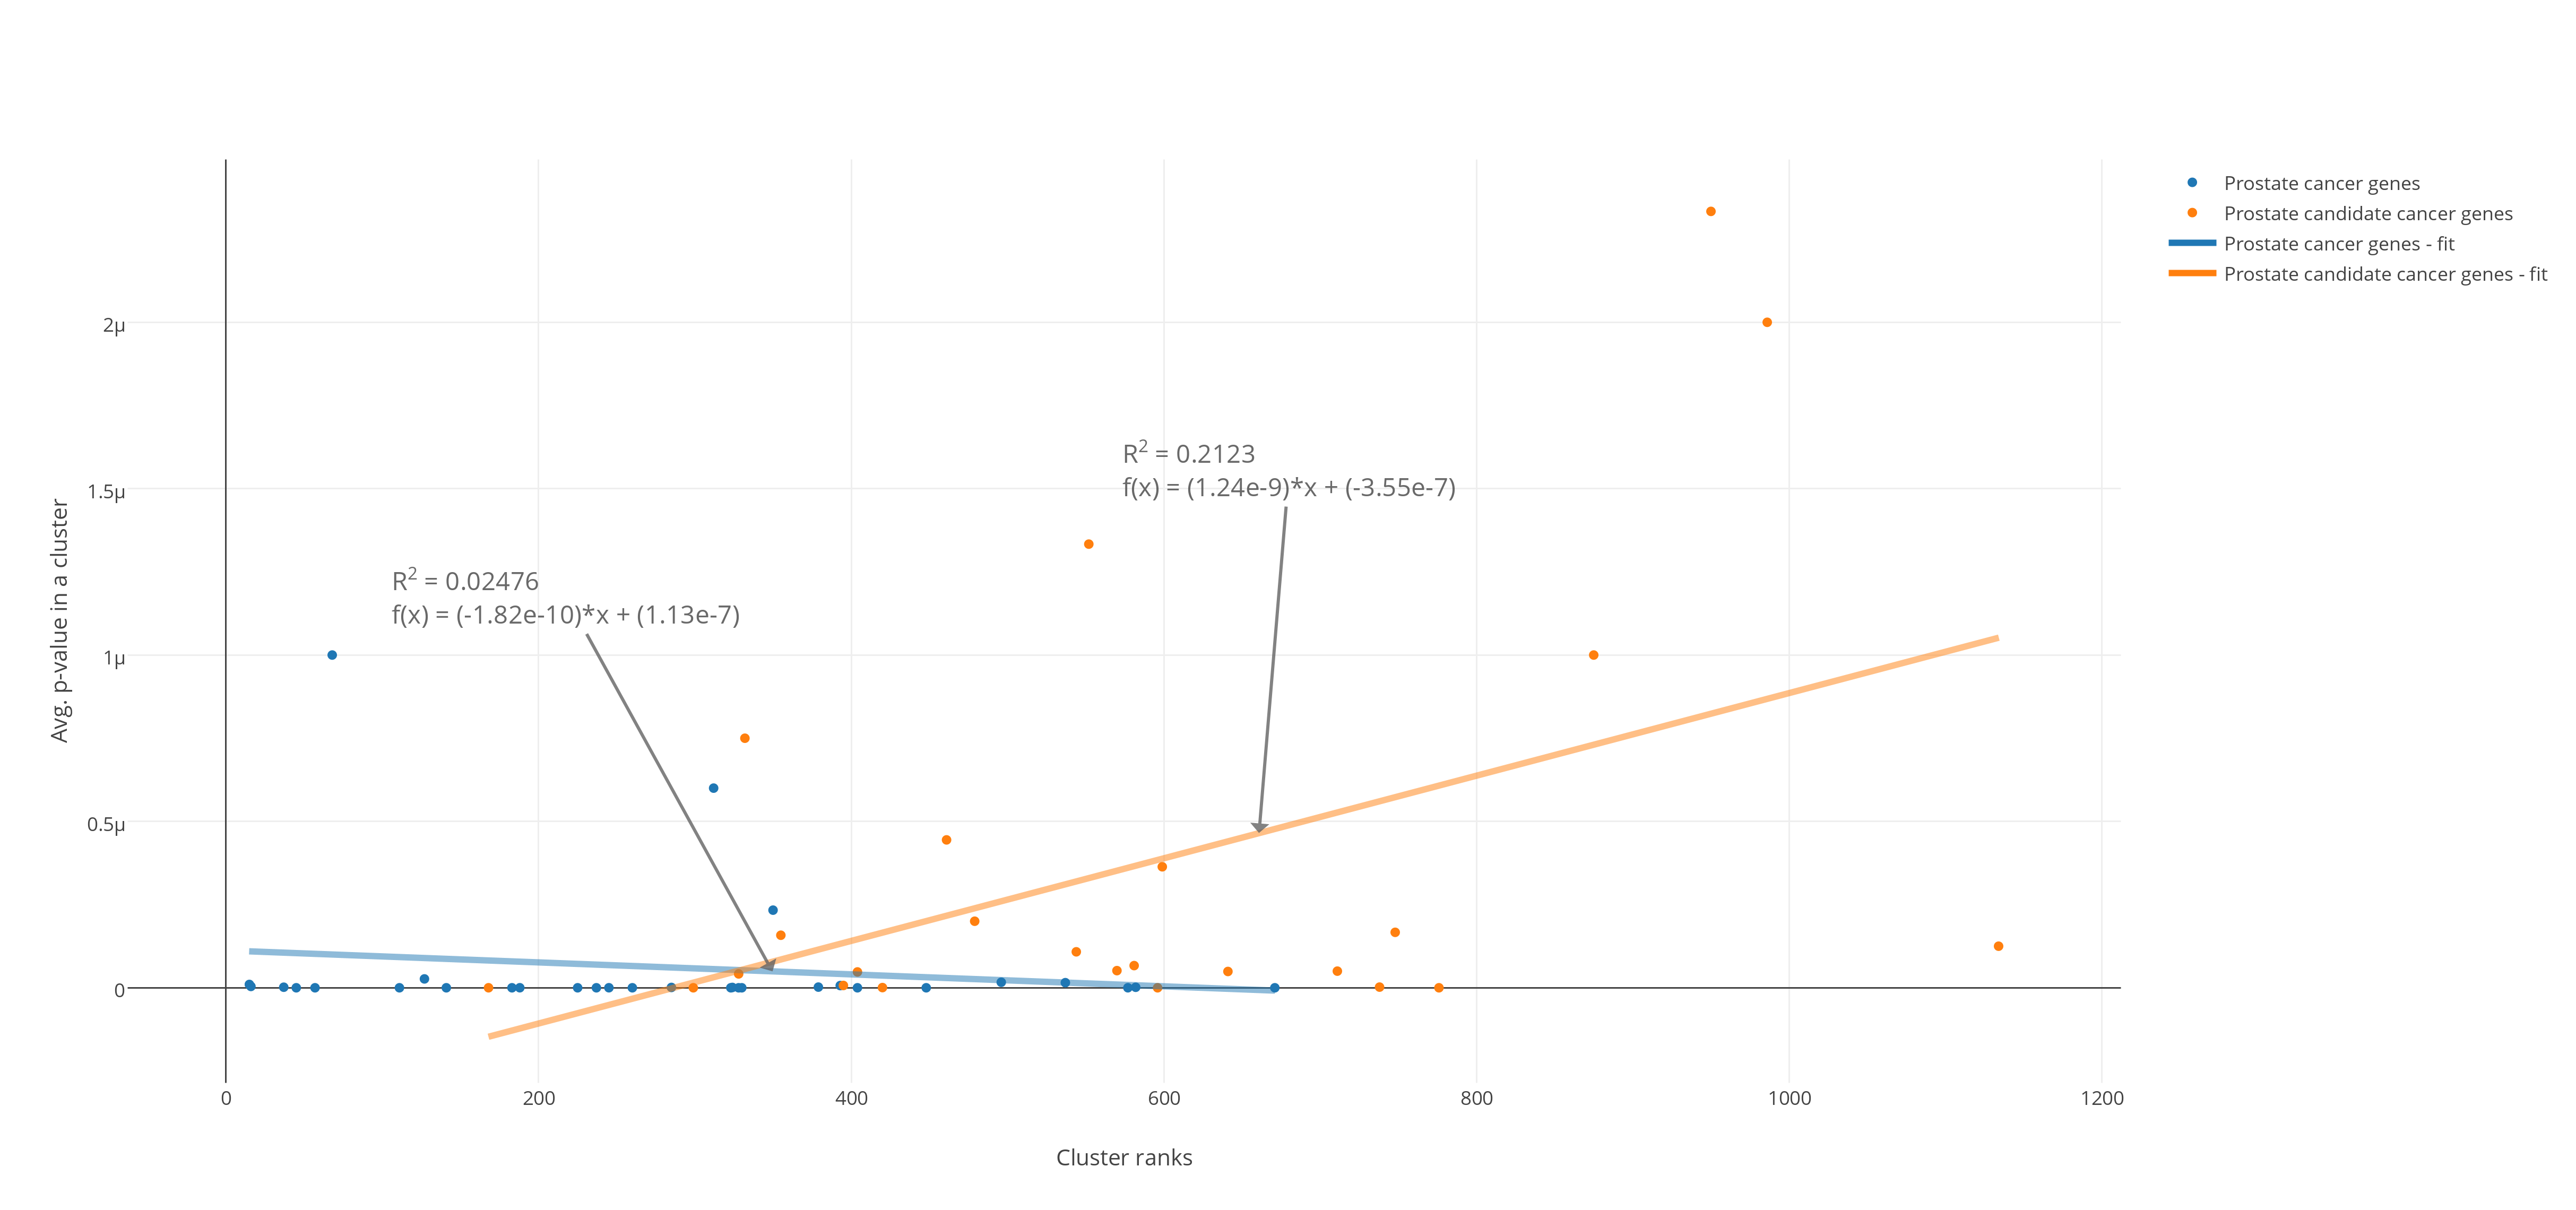
\includegraphics[scale=0.63]{prwp_exp_split}
    \caption{Average distribution of p-values in clusters ranked by PRWP.}
    \label{fig:exp-iref-prwp}
\end{sidewaysfigure}
\begin{sidewaysfigure}
    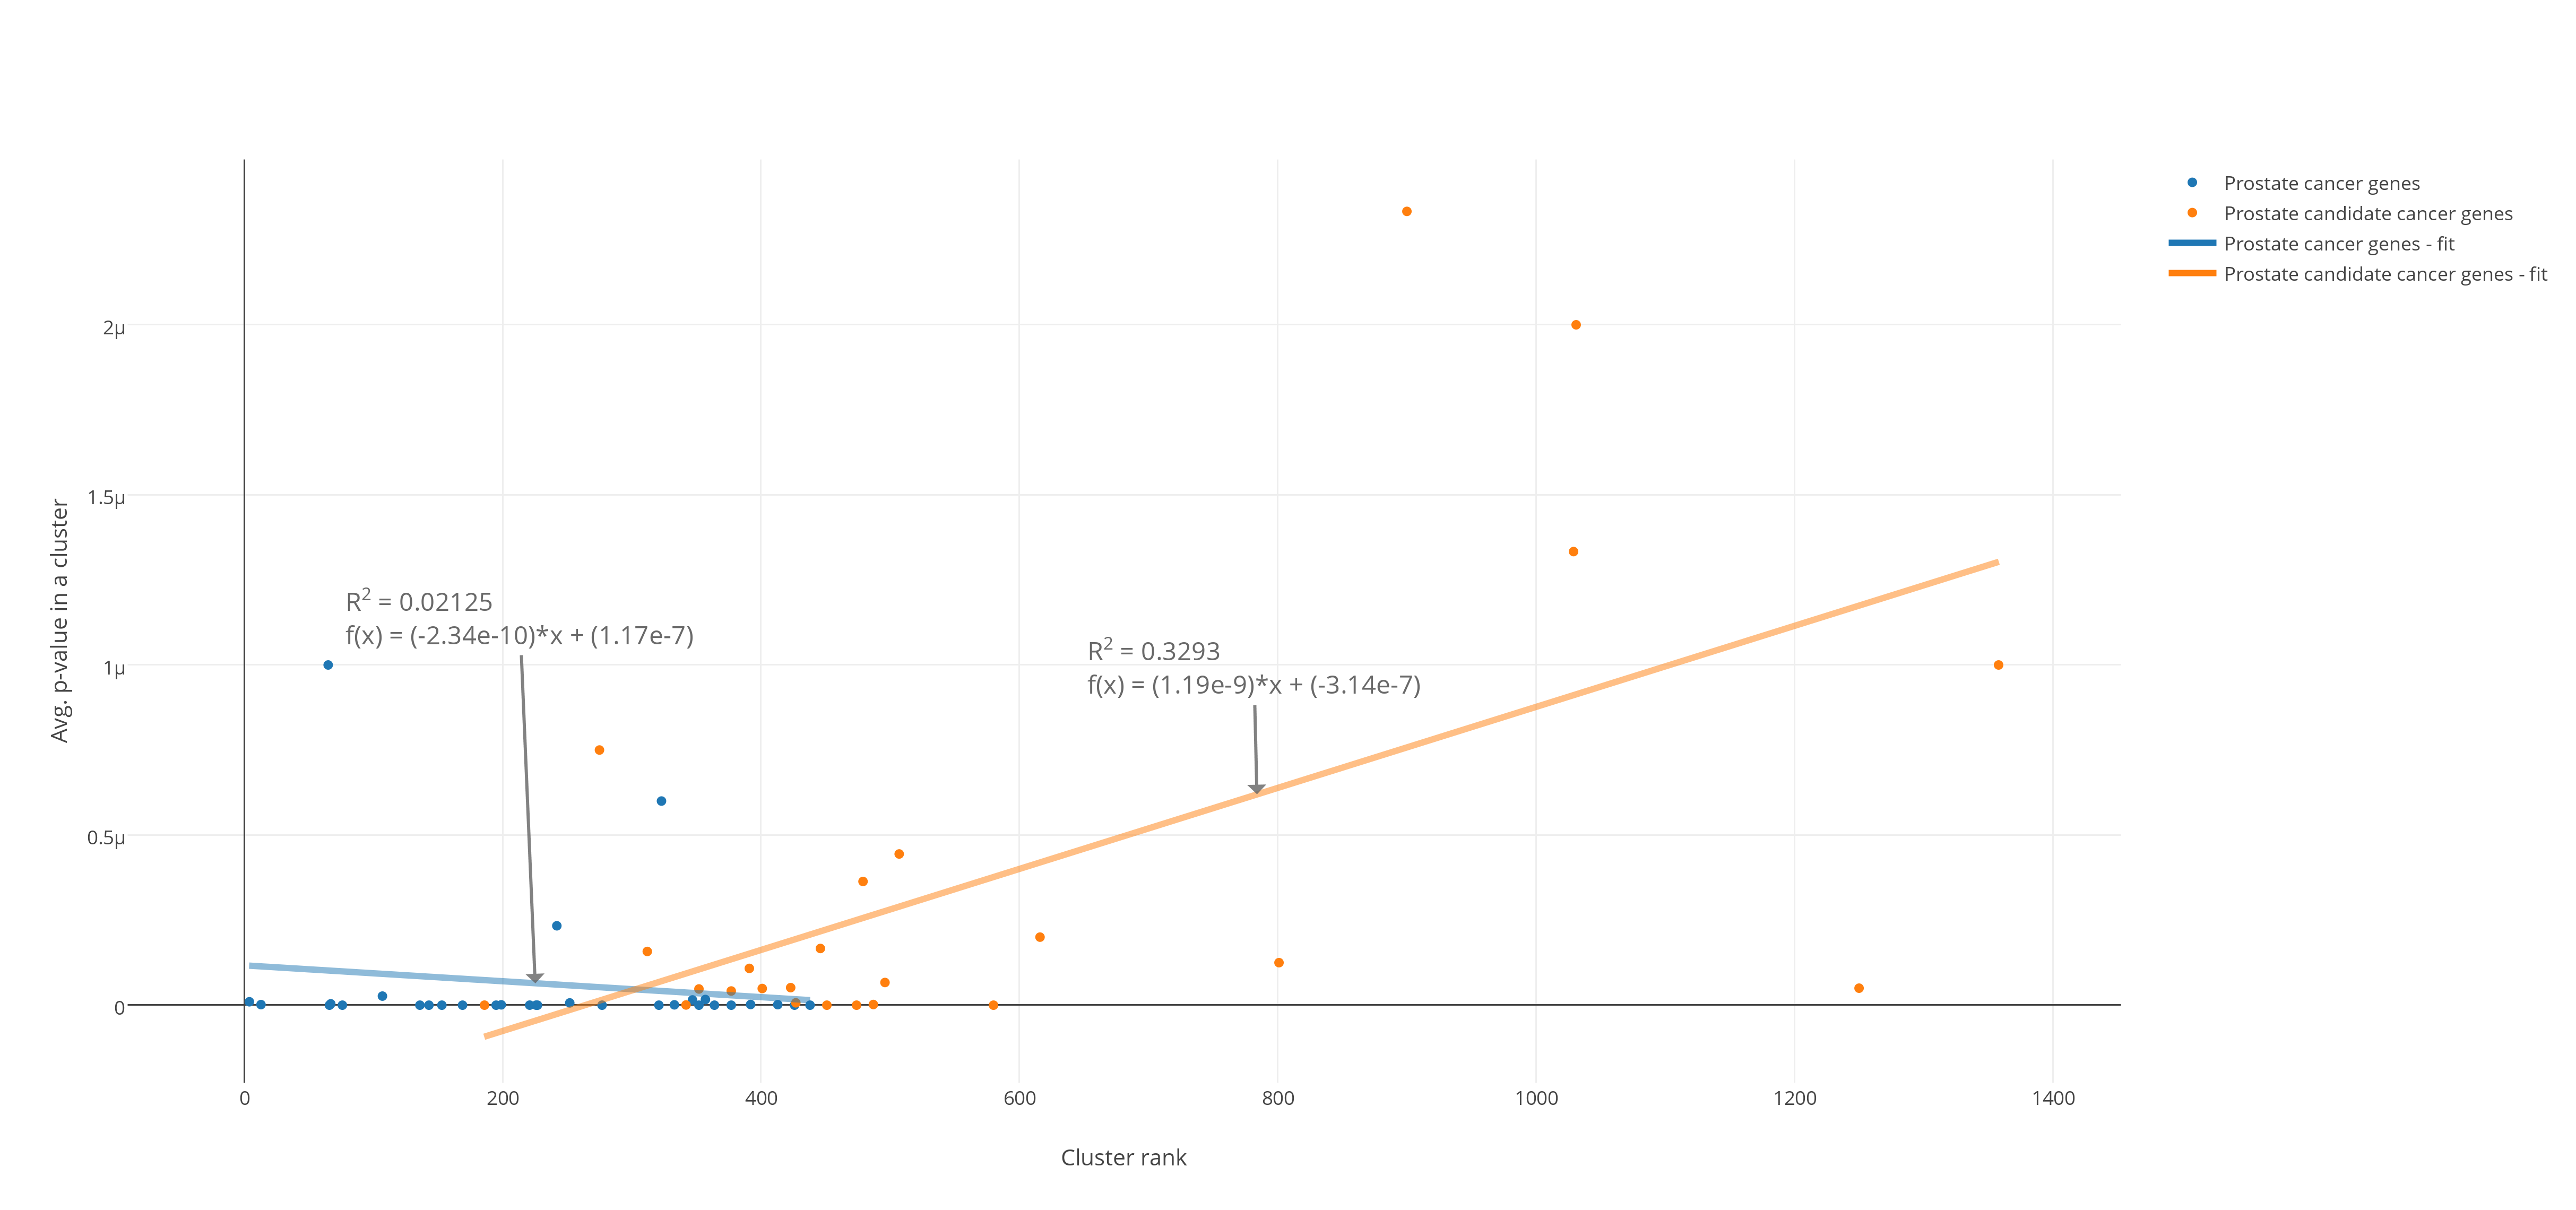
\includegraphics[scale=0.63]{maa_exp_split}
    \caption{Average distribution of p-values in clusters ranked by MAA.}
    \label{fig:exp-iref-maa}
\end{sidewaysfigure}

All of the experimental genes are from experiments and are a result from
genome-wide association studies (GWAS). Each gene in this test data are scored
after p-values from "the most statistically significant SNP within the
block."\cite{distild} in experiments related to prostate cancer. The
\gls{jensen} database has experimental data from both the Catalogue of Somatic
Mutations in Cancer (COSMIC) and DistiLD, but for prostate cancer, only
experimental data from DistiLD was available.

The score for each cluster is calculated from the average p-value from each gene
in the cluster. In contrast to the previous plots, the trend required to
validate \gls{prwp} and \gls{maa} as cluster ranking algorithms for prioritizing
network biomarkers in prostate cancer, is an ascending trend in both genes with
and without prior scores, when ranking clusters from the topmost to the lowest
cluster. An ascending score for the genes with prior scores proves that the
highly ranked clusters have low p-values, which is proof of a low chance of the
null hypothesis being true. Here, the null hypothesis would be that a gene has
no relevance to prostate cancer. The \gls{golden} is based on \gls{dragon} and
DisGeNET scores. The DisGeNET scores are developed as a score based on the
supporting evidence for the context of a gene and a disease being
true\cite{disgenet}. Based on this fact, it is feasible if \gls{prwp} and
\gls{maa} would demonstrate the previously defined trend.

The experimental data has one of the same feats as the manually knowledge
curated data, it is very sparse. As with the previous plots, the genes with
prior scores in a cluster are colored blue, and the ones without prior scores as
orange.

\subsection{PRWP benchmarked by experimentally mined genes}
For \gls{prwp} (figure: \ref{fig:exp-iref-prwp}), there is a trend for descending
p-values for the genes with prior scores in a cluster and an ascending p-value
trend for the genes without prior scores in a cluster. For the genes without
prior scores, this is a feasible result in order to validate Ranklust as a tool
for prioritizing network biomarkers. For the genes with prior scores, there is
a single cluster that seems to be the cause of the descending trend but the
\gls{rsquared} value for the fit of the linear regression is not high.

\subsection{MAA benchmarked by experimentally mined genes}
For \gls{maa} (figure: \ref{fig:exp-iref-maa}), the trends are the same as with
\gls{prwp}, but the trends are more noticeable. For the genes with prior scores,
the descending p-value trend towards the lower ranked clusters are steeper than
the one in the plot for \gls{prwp}, but the \gls{rsquared} score is very low and
the as it is in the \gls{prwp} plot, it seems to be a single cluster that is
responsible for the descending trend in p-values.

\subsection{Conclusion of benchmarking through experimentally mined genes}
As with the manually knowledge curated genes, the experimental genes have
a small sampling size. Also, the trends that would discredit Ranklust's ability
to prioritize network biomarkers is not backed up by very high values of
confidence in terms of \gls{rsquared} values in the linear regression fits. In
this specific case of benchmarking Ranklust, it is a high probability that the
cause of the trend is an outlier in the plot.

\chapter{Comparison of PRWP and MAA to prostate cancer relevant genes}
Using \gls{prwp} and \gls{maa}, 6 final lists of prioritized network biomarkers
for prostate cancer will be presented. These 6 lists will be the result of
3 \gls{prwp} and 3 \gls{maa} ranked clusters from the whole iRefWeb filtered
network with gene names and the scored with the full \gls{golden}. Each of the
3 ranking results from both algorithms will use the same three sets of data,
namely movember, cosmica and lethal.

\section{Using Ranklust to rank the clusters of a network}
The exact workflow of using Ranklust to create the ranks that the test data is
compared to is exactly as explained earlier in both the methods chapter and the
workflow part of this results chapter.

\subsection{Step 1 - create the network and fill it with prior scores}
The network was downloaded from iRefWeb. This network consisted of protein
interactions to create an unweighted and undirected PPI network. These proteins
was then filtered with their corresponding gene names taken from HGNC. Most of
the proteins in the network did not have a corresponding gene name that HGNC
could match, so over half of the interactions was removed.

The \gls{golden} was created as explained earlier, with prostate cancer data
from DisGeNET and \gls{dragon}. The network was uploaded into Cytoscape and
populated with the prior scores. 

\subsection{Step 2 - Clustering the network}
The Markov Cluster algorithm, MCL, was used to cluster the iRefWeb network with
an inflation parameter of 1.8 and 200 iterations. This process took about 15
hours on the High-Performance Computing (HPC) instance Invitro at the University
of Oslo. It used a total of 64 cores, which averaged at a 90-95\% load for the
majority of the time the cluster algorithm ran.

\subsection{Step 3 - Ranking the clusters of the network}
\gls{prwp} and \gls{maa} was ran on the network, choosing only the priors in the
nodes given by the \gls{golden}. The alpha value for \gls{prwp} was set to 0.3
together with 30 max iterations.

\subsection{Step 4 - Exporting cluster ranks from Cytoscape and comparison with test data}
The node table with the results from \gls{prwp} and \gls{maa} was exported to
csv files, cleaned up with python scripts so it would form clusters containing
information about which genes was in which clusters, the rank of the cluster and
which genes in the cluster had a prior score or not.

The test data is in the form of a single column text file where each row
contains the name of a gene. By traversing the ranked list of clusters, four
categories were made from these test data genes. 

The first two was named "test biomarkers" and "test candidates". These two have
in common that they both list genes from the cluster in its column if it is
contained in the test data set of genes. The "test biomarkers" are genes that
both have a prior score and are contained in the test data set of genes. The
"test candidates" are also in the test data set of genes, but they do not have
prior scores.

The next two categories are "remaining biomarkers" and "remaining candidates".
These two categories have in common that neither of them will list genes that
was in the test data set of genes. The difference is that "remaining biomarkers"
have prior scores, and "remaining candidates" have no prior scores.

Each cluster had their genes split into these four categories, represented as
four columns in the next upcoming tables (tables: \ref{tab:prwp-movember}
\ref{tab:maa-movember}, \ref{tab:prwp-cosmic}, \ref{tab:maa-cosmic},
\ref{tab:prwp-lethal}, \ref{tab:maa-lethal}). The last column represents the
rank of the cluster from either \gls{prwp} or \gls{maa}, depending on the table.
From each of these tests, it is displayed the top 10 clusters, which had
a combined amount of genes in either the "test biomarkers" or the "test
candidates" column above 0.

As a comment to each plot, the topmost ranked cluster in each table will be
analyzed when it comes to each of the genes it contains. The genes will be
assigned their functional classification according to PANTHERDB and \gls{jensen}
database\cite{pantherdb,panther,disgenet}.

\section{Prostate cancer genes manually curated from the movember group}
\begin{sidewaystable}
    \begin{tabular}{|l|l|l|l|l|}
        \hline
        \textbf{Rank}
        & \textbf{Test biomarkers}
        & \textbf{Test candidates}
        & \textbf{Remaining biomarkers}
        & \textbf{Remaining candidates} \\
        \hline
        13	& TNFRSF11B	& THBS1	& VEGFA	& - \\
        \hline
        19	& -	& F12	& MMP12	& - \\
        \hline
        25	& F2R	& -	& F2RL1	& PRTN3 \\
        \hline
        28	& -	& RRM2	& MAGEA3,MAGEA1	& DNM1L,PGAM5,SCG3 \\
        \hline
        29	& CEACAM1	& -	& -	& CLEC4M \\
        \hline
        31	& ALOX15B	& -	& -	& ERAL1 \\
        \hline
        46	& SMAD4	& -	& -	& ZMIZ1 \\
        \hline
        48	& STAT6	& -	& ACSL3,IFI16	& TRIM56,TMEM173,SLC39A14 \\
        \hline
        53	& RNASEL	& IQGAP1	& -	& GSPT1,NPHS2 \\
        \hline
        55	& DPP4	& -	& VIP,GHRH,ADCYAP1	& PYY,AVPR1A,GCG,GIP,TAC1,FAP,NPPB \\
        \hline
    \end{tabular}
    \caption{iRefWeb network ranked with PRWP and movember data - matched 254 
    test genes from movember data set out of 271 possible}
    \label{tab:prwp-movember}
\end{sidewaystable}

\textbf{Top ranked cluster ranked with PRWP and tested with Movember data}

\begin{itemize}
    \item TNFRSF11B
        \begin{itemize}
            \item PantherDB subfamily - Tumor necrosis factor receptor
                superfamily, member 11b
            \item \gls{jensen} relation - Relation to several diseases, among
                them cancer (z-score of 4.2)
        \end{itemize}
    \item THBS1
        \begin{itemize}
            \item PantherDB subfamily - Thrombospondin-1
            \item \gls{jensen} relation - Relation to several diseases, among
                them cancer (z-score of 5.0)
        \end{itemize}
    \item VEGFA
        \begin{itemize}
            \item PantherDB subfamily - Vascular endothelial growth factor A
            \item \gls{jensen} relation - Relation to several diseases, among
                them cancer (z-score of 7.5)
        \end{itemize}
\end{itemize}

\begin{sidewaystable}
    \begin{tabular}{|l|l|l|l|l|}
        \hline
        \textbf{Rank}
        & \textbf{Test biomarkers}
        & \textbf{Test candidates}
        & \textbf{Remaining biomarkers}
        & \textbf{Remaining candidates} \\
        \hline
        8	& F2R	& -	& F2RL1	& PRTN3 \\
        \hline
        12	& TNFRSF11B	& THBS1	& VEGFA	& - \\
        \hline
        14	& STAT6	& -	& ACSL3,IFI16	& TRIM56,TMEM173,SLC39A14 \\
        \hline
        20	& -	& F12	& MMP12	& - \\
        \hline
        25	& SMAD4	& -	& -	& ZMIZ1 \\
        \hline
        26	& CD44	& -	& -	& SCYL3 \\
        \hline
        35	& CEACAM1	& -	& -	& CLEC4M \\
        \hline
        57	& BIRC5	& -	& -	& KCNJ6 \\
        \hline
        58	& ALOX15B	& -	& -	& ERAL1 \\
        \hline
        69	& -	& CRIP2	& UXT,RELA,ALPL	& NR1H4,NME5 \\
        \hline
    \end{tabular}
    \caption{iRefWeb network ranked with MAA and movember data - matched 172
    test genes from movember data set out of 271 possible}
    \label{tab:maa-movember}
\end{sidewaystable}

\textbf{Top ranked cluster ranked with MAA and tested with Movember data}

\begin{itemize}
    \item F2R
        \begin{itemize}
            \item PantherDB subfamily - Proteinase-activated receptor 1
            \item \gls{jensen} relation -  Relation to several diseases, among
                them cancer (z-score of 3.3)
        \end{itemize}
    \item F2RL1
        \begin{itemize}
            \item PantherDB subfamily - Proteinase-activated receptor 2
            \item \gls{jensen} relation - Relation to several diseases, among
                them cancer (z-score of 2.4)
        \end{itemize}
    \item PRTN3
        \begin{itemize}
            \item PantherDB subfamily - Myeloblastin
            \item \gls{jensen} relation - Relation to several diseases, cancer
                is not among them
        \end{itemize}
\end{itemize}

\section{Curated prostate cancer genes from the COSMIC database}
\begin{sidewaystable}
    \begin{tabular}{|l|l|l|l|l|}
        \hline
        \textbf{Rank}
        & \textbf{Test biomarkers}
        & \textbf{Test candidates}
        & \textbf{Remaining biomarkers}
        & \textbf{Remaining candidates} \\
        \hline
        6	& TNFAIP3	& -	& RNF14,TAGLN	& - \\
        \hline
        11	& BIRC3	& -	& -	& BIRC2 \\
        \hline
        12	& CXCR4	& -	& -	& CXCL14 \\
        \hline
        17	& -	& DAXX	& TGFBR3,ACVR2A	& TCTEX1D4 \\
        \hline
        18	& RHOA	& -	& AGER	& GMIP \\
        \hline
        24	& -	& ELN	& EFEMP2,SOD3,FBLN5	& - \\
        \hline
        37	& AR	& KMT2A	& MAK,TSPY1	& PKLR,HHAT \\
        \hline
        39	& TOP1	& -	& -	& RCVRN \\
        \hline
        44	& WIF1	& -	& -	& WNT11 \\
        \hline
        46	& SMAD4	& -	& -	& ZMIZ1 \\
        \hline
    \end{tabular}
    \caption{iRefWeb network ranked with PRWP and COSMIC data - matched 423 test
    genes from the COSMIC data set out of 580 possible}
    \label{tab:prwp-cosmic}
\end{sidewaystable}

\textbf{Top ranked cluster ranked with PRWP and tested with COSMIC data}

\begin{itemize}
    \item TNFAIP3
        \begin{itemize}
            \item PantherDB subfamily - Tumor necrosis factor alpha-induced
                protein 3
            \item \gls{jensen} relation - Relation to several diseases, among them
                cancer (z-score of 3.3)
        \end{itemize}
    \item RNF14
        \begin{itemize}
            \item PantherDB subfamily - Ubiquitin-protein ligase
            \item \gls{jensen} relation - Relation to several diseases, among them
                specificly prostate cancer (z-score of 3.6)
        \end{itemize}
    \item TAGLN
        \begin{itemize}
            \item PantherDB subfamily - Transgelin
            \item \gls{jensen} relation - Relation to several diseases, among them
                cancer (z-score of 4.2)
        \end{itemize}
\end{itemize}
\begin{sidewaystable}
    \begin{tabular}{|l|l|l|l|l|}
        \hline
        \textbf{Rank}
        & \textbf{Test biomarkers}
        & \textbf{Test candidates}
        & \textbf{Remaining biomarkers}
        & \textbf{Remaining candidates} \\
        \hline
        1	& TNFAIP3	& -	& RNF14,TAGLN	& - \\
        \hline
        10	& RHOA	& -	& AGER	& GMIP \\
        \hline
        13	& AR	& KMT2A	& MAK,TSPY1	& PKLR,HHAT \\
        \hline
        14	& STAT6,ACSL3	& -	& IFI16	& TRIM56,TMEM173,SLC39A14 \\
        \hline
        15	& -	& DAXX	& TGFBR3,ACVR2A	& TCTEX1D4 \\
        \hline
        17	& BIRC3	& -	& -	& BIRC2 \\
        \hline
        19	& -	& SUFU	& PIAS1	& - \\
        \hline
        25	& SMAD4	& -	& -	& ZMIZ1 \\
        \hline
        29	& SET	& -	& -	& TAF1C \\
        \hline
        37	& TOP1	& -	& -	& RCVRN \\
        \hline
    \end{tabular}
    \caption{iRefWeb network ranked with MAA and COSMIC data - matched 277 test
    genes from the COSMIC data set out of 580 possible}
    \label{tab:maa-cosmic}
\end{sidewaystable}

\textbf{Top ranked cluster ranked with MAA and tested with COSMIC data}

\begin{itemize}
    \item TNFAIP3
        \begin{itemize}
            \item PantherDB subfamily - Tumor necrosis factor alpha-induced
                protein 3
            \item \gls{jensen} relation - Relation to several diseases, among them
                cancer (z-score of 3.3)
        \end{itemize}
    \item RNF14
        \begin{itemize}
            \item PantherDB subfamily - Ubiquitin-protein ligase
            \item \gls{jensen} relation - Relation to several diseases, among them
                specificly prostate cancer (z-score of 3.6)
        \end{itemize}
    \item TAGLN
        \begin{itemize}
            \item PantherDB subfamily - Transgelin
            \item \gls{jensen} relation - Relation to several diseases, among them
                cancer (z-score of 4.2)
        \end{itemize}
\end{itemize}

\section{Proven prostate cancer genes that resulted in lethal outcome for the patient}
\begin{sidewaystable}
    \begin{tabular}{|l|l|l|l|l|}
        \hline
        \textbf{Rank}
        & \textbf{Test biomarkers}
        & \textbf{Test candidates}
        & \textbf{Remaining biomarkers}
        & \textbf{Remaining candidates} \\
        \hline
        25	& F2R	& -	& F2RL1	& PRTN3 \\
        \hline
        28	& -	& RRM2	& MAGEA3, MAGEA1	& DNM1L, PGAM5, SCG3 \\
        \hline
        31	& ALOX15B	& -	& -	& ERAL1 \\
        \hline
        55	& DPP4	& -	& VIP, GHRH, ADCYAP1	& PYY, AVPR1A, GCG, GIP, TAC1, FAP, NPPB \\
        \hline
        79	& BIRC5	& -	& -	& KCNJ6 \\
        \hline
        88	& SERPINA3	& -	& KLK4	& CTRC, GZMM, SGCD \\
        \hline
        91	& -	& CRIP2	& UXT, RELA, ALPL	& NR1H4, NME5 \\
        \hline
        92	& CCNB1	& UBE2C	& -	& UBE3D \\
        \hline
        114	& JAG1	& -	& -	& NEURL1, CD46 \\
        \hline
        120	& -	& CYB5A	& CYP17A1, CYP3A4, CYP3A5, CYP2E1	& CYP4F2, CYP4A11 \\
        \hline
    \end{tabular}
    \caption{iRefWeb network ranked with PRWP and lethal prostate cancer data
    - matched 99 test genes form the lethal prostate cancer data set out of 157
possible}
    \label{tab:prwp-lethal}
\end{sidewaystable}

\textbf{Top ranked cluster ranked with PRWP and tested with Lethal prostate cancer data}

\begin{itemize}
    \item F2R
        \begin{itemize}
            \item PantherDB subfamily - Proteinase-activated receptor 1
            \item \gls{jensen} relation -  Relation to several diseases, among
                them cancer (z-score of 3.3)
        \end{itemize}
    \item F2RL1
        \begin{itemize}
            \item PantherDB subfamily - Proteinase-activated receptor 2
            \item \gls{jensen} relation - Relation to several diseases, among
                them cancer (z-score of 2.4)
        \end{itemize}
    \item PRTN3
        \begin{itemize}
            \item PantherDB subfamily - Myeloblastin
            \item \gls{jensen} relation - Relation to several diseases, cancer
                is not among them
        \end{itemize}
\end{itemize}

\begin{sidewaystable}
    \begin{tabular}{|l|l|l|l|l|}
        \hline
        \textbf{Rank}
        & \textbf{Test biomarkers}
        & \textbf{Test candidates}
        & \textbf{Remaining biomarkers}
        & \textbf{Remaining candidates} \\
        \hline
        8	& F2R	& -	& F2RL1	& PRTN3 \\
        \hline
        57	& BIRC5	& -	& -	& KCNJ6 \\
        \hline
        58	& ALOX15B	& -	& -	& ERAL1 \\
        \hline
        69	& -	& CRIP2	& UXT,RELA,ALPL	& NR1H4,NME5 \\
        \hline
        79	& -	& RRM2	& MAGEA3,MAGEA1	& DNM1L,PGAM5,SCG3 \\
        \hline
        92	& CCNB1	& UBE2C	& -	& UBE3D \\
        \hline
        105	& JAG1	& -	& -	& NEURL1,CD46 \\
        \hline
        106	& DPP4	& -	& VIP,GHRH,ADCYAP1	& PYY,AVPR1A,GCG,GIP,TAC1,FAP,NPPB \\
        \hline
        109	& SERPINA3	& -	& KLK4	& CTRC,GZMM,SGCD \\
        \hline
        112	& -	& CYB5A	& CYP17A1,CYP3A4,CYP3A5,CYP2E1	& CYP4F2,CYP4A11 \\
        \hline
    \end{tabular}
    \caption{iRefWeb network ranked with MAA and lethal prostate cancer data
    - matched 66 test genes form the lethal prostate cancer data set out of 157
possible}
    \label{tab:maa-lethal}
\end{sidewaystable}

\textbf{Top ranked cluster ranked with MAA and tested with Lethal prostate cancer data}

\begin{itemize}
    \item F2R
        \begin{itemize}
            \item PantherDB subfamily - Proteinase-activated receptor 1
            \item \gls{jensen} relation -  Relation to several diseases, among
                them cancer (z-score of 3.3)
        \end{itemize}
    \item F2RL1
        \begin{itemize}
            \item PantherDB subfamily - Proteinase-activated receptor 2
            \item \gls{jensen} relation - Relation to several diseases, among
                them cancer (z-score of 2.4)
        \end{itemize}
    \item PRTN3
        \begin{itemize}
            \item PantherDB subfamily - Myeloblastin
            \item \gls{jensen} relation - Relation to several diseases, cancer
                is not among them
        \end{itemize}
\end{itemize}

\section{Final results from testing PRWP and MAA against prostate cancer test data}
Comparing \gls{prwp} to \gls{maa} clearly shows that \gls{prwp} is better at
identifying and prioritizing network biomarkers for prostate cancer. This
conclusion is based on which of the two ranking algorithms that had the highest
percentage of genes in the cluster ranks that was found in the test gene sets.
The main difference between \gls{prwp} and \gls{maa} is, as mentioned earlier,
that \gls{prwp} takes network structure into consideration when ranking nodes in
the network, and as a result, manages to give meaningful scores to a greater
number of clusters than \gls{maa}.

\begin{table}[H]
    \begin{tabular}{c l c c c}
        & \textbf{Data set} & \textbf{Hits} & \textbf{Possible hits}
                           & \textbf{Percentage} \\
        \hline
        \multirow{3}{*}{\rotatebox{90}{PRWP}}
        & Movember & 254 & 271 & 93.7 \\
        & COSMIC & 423 & 580 & 72.3 \\
        & Lethal & 99 & 157 & 63.1 \\
        \hline
        \multirow{3}{*}{\rotatebox{90}{MAA}}
        & Movember & 172 & 271 & 64.5 \\
        & COSMIC & 277 & 580 & 47.8 \\
        & Lethal & 66 & 157 & 43.0 \\
        \hline
    \end{tabular}
    \caption{Test data hits for PRWP and HITS}
    \label{tab:final}
\end{table}

Also, the are two of the topmost ranked clusters that occur in several of the
test data sets across ranking algorithms. 

These first cluster consist of the following genes: F2R, F2RL1 and PRTN3. This
cluster was the topmost ranked cluster by both \gls{prwp} and \gls{maa}, that
contained genes from the Lethal prostate cancer data set. \gls{maa} also had it
listed as the topmost ranked cluster, that contained genes from the Movember
data set.

These second cluster consist of the following genes: TNFAIP3, RNF14 and TAGLN.
This cluster was the topmost ranked cluster by both \gls{prwp} and \gls{maa},
that contained genes from the COSMIC test data set.

The cluster that contained F2R, F2RL1 and PRTN3 was the topmost ranked cluster
in 3 out of the 6 cases with test data. The cluster that contained TNFAIP3,
RNF14 and TAGLN occured 2 out of 6 times with the test data. The last topmost
ranked cluster appeared in the Movember data set and was ranked by \gls{prwp}.
It contained the genes TNFRSF11B, THBS1 and VEGFA.

\part{Analysis}
Analysis...

\part{Discussion and conclusion}
\label{pa:conclusion}
\chapter{Discussion}
\section{Network handling}
If the whole network could receive a change in a single aspect that would make
for a better network to rank clusters in, it would be the direction of the
edges. The ranking algorithms used can all come to useful results with
undirected edges, but directed edges take better advantage of how \gls{pr},
\gls{prwp}, \gls{hits} are meant to be used.

\subsection{Clustering}
The clusters could to a greater degree have been filtered more strictly. The
average cluster size was around 8.8 nodes (Table \ref{tab:mcl-inflation}), the
biggest cluster consisted if over 900 nodes, and the smallest ones were 2.0 
nodes in size. Removing the smaller clusters with only 2 genes has been done by
other researchers because of the low likeliness of a protein complex with only
2 genes to have a significant impact on disease status. The biggest cluster
might also be removed due to its large size when compared to the average. Such
a large cluster has a good chance of not being realistically compartmentalized
into a protein complex, and can skew the results in either the direction of
false positives or false negatives.

\subsection{Ranking}
Ranking the cluster-created network could have been done instead of or
complimentary to the network which only received cluster attributes as a sign
of clustering, and had no perturbation of the edges as a result of clustering.

Adjusting the alpha parameter of \gls{prwp} to higher values as 0.8 instead of 0.3 would also
give interesting information. Had the cross-validation with \gls{prwp} 
been done with 0.8, and resulted in a linear regression fit
(Figure \ref{fig:irefweb-prwp}) that would have had a less descending trend of
candidate cancer genes throughout the cluster ranks, it would be significant
proof of the network structure having a bigger effect on the rankings than the
priors scores.

\chapter{Conclusion}
\section{Future work}
\subsection{General improvements}
I have used an undirected network, which is not the preferred type to use with
PageRank, but it works. An idea could be to use KEGG pathways\cite{kegg}, which
has the option of downloading directed networks of several types.
STRING\cite{str} also has some directed network information, together with
weights. Because of STRINGs size, utilizing a Neo4J database to perform the
ranking algorithms could be a better option than directly having Cytoscape do
all of the heavy computations.

In the future, maybe a database with complete protein complexes could exclude
the need for clustering and provide different ways of ranking them based on
query criteria.

Other ranking algorithms than PageRank could also have been used. There are
numerous variations based off of this well known algorithm, for example NetRank
and GeneRank\cite{netrank,generank}. Not all of these PageRank variants are
intended to be used with PPI networks, but they can in many cases be modified to
fit this specific purpose.

In Ranklust, the average score in the nodes becomes the cluster score. PageRank
was used to combine prior knowledge of cancer genes and network structure to
prioritize network biomarers in prostate cancer. Taking the structure of the
network in higher consideration and maybe consider the distance between the
nodes to have an effect on the result could be a contribution to the PageRank
algorithm. Also, going the other way and increase the significance of the prior
scores added to the nodes in the network could help to get a better segregated
result of which clusters are related to cancer and not. For example, PRWP used
an alpha value of 0.3 because of earlier experiments in ranking biological
networks with PageRank had good results with it. What if the alpha value was set
to 0.8 and give the prior scores in the node a higher degree of bias?

\subsection{Minor features to complement Ranklust/clusterMaker2}
A compiled list of all considered features and tweaks in the Ranklust
contribution to clusterMaker2

\begin{itemize}
    \item User can specify what direction the ranking algorithm should consider
        for the graph
\end{itemize}

\subsection{Ranking through Neo4J}
ClusterMaker2 does every calculation within Cytoscape. There exists another way
of doing large and complex calculations, especially when it comes to algorithms
that focus on edge information in the network. CyNeo4j\cite{cyneo4j} is
a Cytoscape App that can realise this idea. It supports import/export of data
with a Neo4J\cite{neo4j} database. The original CyNeo4J Github-repository does
not support user authentication at the moment, but during the discussion about
what ranking algorithm should be used, Neo4J was an alternative. It resulted in
a git fork\cite{git-fork} of the CyNeo4J repository and simple user/password
authentication was added.

\subsection{Data communication}
Data communication between the Neo4J database server and the Cytoscape instance
is done through the CyNeo4J app to Cytoscape \cite{cyneo4j}. CyNeo4J is a
Cytoscape app that was developed during the Google Summer Code 2014 arrangement.
It supports connecting to a Neo4J instance, as well as syncing data up and down
from and to the database server. One thing it did not support was authentication
on Neo4J servers. Not having authentication is a serious problem, so we
implemented a simple way of getting access to the database server by providing a
possibility to insert username and password at the same time the user has to
provide a URL to the Neo4J database server instance. Implementation-wise, this
only required an extra header to be included in each http request going to the
password protected Neo4J database server instance. Every request used the static
\textbf{Request} class to Get/Post/Put HTTP requests to the Neo4J database
server instance. Except for creating the Auth64 encoded information, the
refactor looked something along these lines in all of the files.

Before:
\begin{lstlisting}[frame=single,language=Java]
Request req = Request.Post(url)
        .bodyString(call.getPayload(), ContentType.APPLICATION_JSON);
\end{lstlisting}

After:
\begin{lstlisting}[frame=single,language=Java]
Request req = Request.Post(url)
        .addHeader("Authorization", auth64EncodedInfo)
        .bodyString(call.getPayload(), ContentType.APPLICATION_JSON);
\end{lstlisting}

Synchronization time between Neo4J and Cytoscape through the CyNeo4J app is a
huge timesink. As of now, the time it takes to populate an empty Cytoscape
network with the gene information from STRING is about 2 hours, though on a slow
laptop. This could be shortened by exporting the Neo4J data with GraphML and
into Cytoscape. Because after the initial data is inside Cytoscape, updates to
the Neo4J instance goes much faster.

The CyNeo4J also uses a legacy HTTP library to get information from the Neo4J
database \cite{legacy-neo4j}. It is possible that the performance increases with
the new library \cite{transactional-neo4j}. The new library supports creating
transactions, which implicit gives support for rollbacks in case something goes
wrong with the query.

A future improvement to the CyNeo4J app could be to change the communication
between Neo4J and Cytoscape to be done in GraphML and not Cypher. This is
because through this whole process of importing and exporting data from and to
Neo4J, GraphML has shown itself to be a superior format over Cypher. Though, to
this day, direct queries to a running Neo4J instance has to be done in Cypher,
and is not possible in GraphML.

\section{Final results from identifying and prioritizing network biomarkers in prostate cancer}
In the three unique clusters that had the topmost ranks in the results from
testing \gls{prwp} and \gls{maa} against several data test sources related to
prostate cancer, every gene in these clusters was related to cancer, except for
1, PRTN3. \gls{maa} ranked the cluster that contained PRTN3 higher than clusters
where all of the genes were related to cancer, when checked in the \gls{jensen}
database. 

\backmatter{}
\printbibliography
\end{document}
